\subsection{Statistical Methods}
We derive upper limits on the product of the Higgs boson production
cross section and the $\Hi \to \WW$ branching fraction,
$\sigma_{\rm{H}} \times $BR($\Hi \to \WW)$, with respect to the SM
expectation, i.e. $\sigma^{95\%}/\sigma^{SM}$. Two different
statistical methods are used to report results. The first method is
based on Bayesian inference~\cite{bayesian} and the second one, known
as $CL_{s}$, is the modified frequentist approach~\cite{cls1,cls2}.

The likelihood function is defined as:
\begin{eqnarray}
  L(\rm{data}|\mu,\theta)&=&\rm{Poisson}(\rm{data}|\mu\cdot s(\theta)+b(\theta))\cdot p(\tilde{\theta}|\theta) \nonumber\\
 &=&\prod_i\frac{(\mu s_i+b_i)^{n_i}}{n_i!}e^{-\mu s_i-b_i}\cdot p(\tilde{\theta}|\theta)
\label{eq:likelihood}
\end{eqnarray}
where $\mu$ is the signal strength modifier which is often reported in
the upper limit results as a ratio of the cross-section upper limit
over the standard model cross-section and $\theta$ represents a full
set of nuisance parameters that are used to incorporate systematic
uncertainties. 

The first method (Bayesian) is based on interpreting the likelihood
(Eq.~\ref{eq:likelihood}) as a probability distribution function with
a flat prior for the signal strength and a set of pdfs for nuisance
parameters, which are often approximated with the log-normal
distribution. Integrating over the nuisance parameters we find the
upper limit for the signal strength.

For $CL_{s}$ method the test statistic is defined as a likelihood
ratio:
\begin{equation}
\tilde{q_\mu}=-2\log\frac{L(\rm{data}|\mu,\hat\theta_\mu)}{L(\rm{data}|\hat\mu,\hat\theta)}
\end{equation}
where the numerator corresponds to the maximum likelihood for given
``data'' and $\mu$ profiling over the nuisance parameters and the
denominator corresponds to the maximum likelihood for given ``data''
profiling over the nuisance parameters and $\mu$. This test statistic
differs from the ones used at LEP (no profiling of systematic errors)
and at Tevatron (the denominator likelihood uses $\mu=0$ and only
systematic errors are profiled).

The results obtained using the two methods may differ but in most cases
they are very close. To perform the computation of the limits, the
software packages
\texttt{RooStats}~\cite{rootstat} and \texttt{LandS}~\cite{lands} have 
been used.

\subsection{Background Estimation}

The estimation of the backgrounds follows the strategies described in
Section~\ref{sec:backgrounds}. As mentioned at the begining of the 
document, we are totally/partially missing $\wgamma$, $\wgamma^{*}$ and $\WZ$
in simulation. Thus, Monte Carlo yields and data/MC scale factors 
are preliminary.

First we estimate the $\dyll$ (Table~\ref{tab:dy}). As it was seen
before the simulation significantly underestimates this type of
background. It is important to keep in mind that $\WZ$ and $\ZZ$ 
contributions in the $\Z$-peak region are sizable, so the method depends
on the Monte Carlo simulation of these processes. It is not a problem
since the uncertainties on these di-boson contributions in the Z-peak
region are small compared with the systematic uncertainties of the
R-value extraction and the statistical uncertainties on the number of
the events in Z-peak region.

The $\Wjets$ background contribution is summarized in Table~\ref{tab:fake_est}. 
The same sign closure test in the 0-jet bin finds 14 events in data while 
the background expectation is $13 \pm 3~(stat.)$.

The top background estimation is shown in
Table~\ref{tab:ttbar_est}. The scale factors are consistent with unity 
within the current large statistical uncertainties.

With these results, we compare the yields after the $\WW$ preselection 
in data and MC with min-MET(Table~\ref{tab:wwselection_all_minmet}) and 
DY MVA(Table~\ref{tab:wwselection_all_dymva}). Higgs contribution at
\WW\ selection level is negligible for not excluded Higgs mass
hypotheses. For the signal extraction we estimate the \WW\ background
contribution in data looking at events with large di-lepton mass, i.e.
$m_{ll}>100$~\GeV{} (Table~\ref{tab:ww_est}). 
We find roughly 37\%(25\%) more \WW\ events in data than in Monte Carlo for 0(1)-jet
case. The large discrepancy might be due to missing some Mote Carlo samples. 
We will update the result later including them.  
Figures~\ref{fig:ww_ptmax}-\ref{fig:ww_deltaphi} show a few key distributions at \WW\ selection level.

%%%%%%%%%%%%%%%%%%%%%%%%%%%%%%
\begin{table}
\begin{center}
\begin{tabular}{c c c c c c}
\hline
\hline
\multicolumn{5}{c}{0-jet} \\
\hline
       mass & $N_{in}$(data)        & $R_{out/in}$        & $N_{out}$(data)  & $N_{out}$ (MC) \\ 
\hline
       WW & 68.8 $\pm$ 14.2 & 0.29 $\pm$ 0.03 $\pm$ 0.04 & 19.9 $\pm$ 4.5 $\pm$ 2.9 & 4.69 $\pm$ 0.89 \\
 115 \GeV & 17.6 $\pm$ 5.7 & 0.37 $\pm$ 0.04 $\pm$ 0.04 & 6.5 $\pm$ 2.2 $\pm$ 0.7 & 1.46 $\pm$ 0.59 \\
 120 \GeV & 16.8 $\pm$ 6.2 & 0.37 $\pm$ 0.04 $\pm$ 0.04 & 6.2 $\pm$ 2.4 $\pm$ 0.6 & 1.51 $\pm$ 0.59 \\
 125 \GeV & 12.2 $\pm$ 5.3 & 0.60 $\pm$ 0.07 $\pm$ 0.13 & 7.3 $\pm$ 3.3 $\pm$ 1.6 & 1.51 $\pm$ 0.59 \\
 130 \GeV & 7.2 $\pm$ 4.4 & 1.14 $\pm$ 0.16 $\pm$ 0.37 & 8.3 $\pm$ 5.2 $\pm$ 2.7 & 1.07 $\pm$ 0.49 \\
 135 \GeV & 8.0 $\pm$ 4.5 & 1.07 $\pm$ 0.15 $\pm$ 0.42 & 8.6 $\pm$ 5.0 $\pm$ 3.4 & 0.97 $\pm$ 0.48 \\
 140 \GeV & 8.2 $\pm$ 4.0 & 0.96 $\pm$ 0.14 $\pm$ 0.39 & 7.8 $\pm$ 4.0 $\pm$ 3.2 & 0.97 $\pm$ 0.48 \\
 145 \GeV & 14.8 $\pm$ 4.8 & 0.68 $\pm$ 0.11 $\pm$ 0.39 & 10.2 $\pm$ 3.7 $\pm$ 5.7 & 1.90 $\pm$ 0.54 \\
 150 \GeV & 8.9 $\pm$ 4.7 & 0.26 $\pm$ 0.08 $\pm$ 0.16 & 2.3 $\pm$ 1.4 $\pm$ 1.4 & 1.26 $\pm$ 0.50 \\
 160 \GeV & 2.6 $\pm$ 3.2 & 0.40 $\pm$ 0.15 $\pm$ 0.70 & 1.0 $\pm$ 1.3 $\pm$ 1.8 & 0.88 $\pm$ 0.46 \\
 170 \GeV & 1.0 $\pm$ 2.5 & 0.21 $\pm$ 0.10 $\pm$ 1.30 & 0.2 $\pm$ 0.5 $\pm$ 1.3 & 0.28 $\pm$ 0.09 \\
 180 \GeV & 1.0 $\pm$ 2.9 & 0.16 $\pm$ 0.07 $\pm$ 0.45 & 0.2 $\pm$ 0.5 $\pm$ 0.4 & 0.52 $\pm$ 0.19 \\
 190 \GeV & 4.0 $\pm$ 4.6 & 0.25 $\pm$ 0.08 $\pm$ 0.17 & 1.0 $\pm$ 1.2 $\pm$ 0.7 & 0.55 $\pm$ 0.19 \\
 200 \GeV & 7.1 $\pm$ 6.0 & 0.17 $\pm$ 0.05 $\pm$ 0.05 & 1.2 $\pm$ 1.1 $\pm$ 0.4 & 0.55 $\pm$ 0.19 \\
 250 \GeV & 18.9 $\pm$ 8.0 & 0.05 $\pm$ 0.01 $\pm$ 0.02 & 1.0 $\pm$ 0.5 $\pm$ 0.5 & 0.68 $\pm$ 0.43 \\
 300 \GeV & 10.9 $\pm$ 6.1 & 0.13 $\pm$ 0.04 $\pm$ 0.03 & 1.5 $\pm$ 0.9 $\pm$ 0.3 & 0.20 $\pm$ 0.09 \\
\vspace{-3mm} && \\
\hline
\hline
\multicolumn{5}{c}{1-jet} \\
\hline
       mass & $N_{in}$(data)        & $R_{out/in}$        & $N_{out}$(data)  & $N_{out}$ (MC) \\ 
\hline
  WW      & 112.6 $\pm$ 12.1 & 0.24 $\pm$ 0.02 $\pm$ 0.05 & 26.8 $\pm$ 3.5 $\pm$ 5.7  & 7.04 $\pm$ 1.30 \\
 115 \GeV & 5.2 $\pm$ 2.5 & 0.41 $\pm$ 0.11 $\pm$ 0.23 & 2.1 $\pm$ 1.2 $\pm$ 1.2  & 0.00 $\pm$ 0.00 \\
 120 \GeV & 5.6 $\pm$ 2.7 & 0.41 $\pm$ 0.11 $\pm$ 0.23 & 2.3 $\pm$ 1.3 $\pm$ 1.3  & 0.00 $\pm$ 0.00 \\
 125 \GeV & 5.0 $\pm$ 2.5 & 0.56 $\pm$ 0.16 $\pm$ 0.33 & 2.8 $\pm$ 1.6 $\pm$ 1.6  & 0.00 $\pm$ 0.00 \\
 130 \GeV & 4.3 $\pm$ 2.2 & 0.84 $\pm$ 0.26 $\pm$ 0.49 & 3.7 $\pm$ 2.2 $\pm$ 2.1  & 0.00 $\pm$ 0.00 \\
 135 \GeV & 4.2 $\pm$ 2.2 & 0.82 $\pm$ 0.26 $\pm$ 0.48 & 3.5 $\pm$ 2.1 $\pm$ 2.0  & 0.00 $\pm$ 0.00 \\
 140 \GeV & 3.2 $\pm$ 2.0 & 0.73 $\pm$ 0.24 $\pm$ 0.39 & 2.3 $\pm$ 1.7 $\pm$ 1.3  & 0.00 $\pm$ 0.00 \\
 145 \GeV & 19.0 $\pm$ 4.7 & 0.30 $\pm$ 0.03 $\pm$ 0.21 & 5.7 $\pm$ 1.6 $\pm$ 3.9  & 2.04 $\pm$ 0.66 \\
 150 \GeV & 35.2 $\pm$ 6.3 & 0.17 $\pm$ 0.03 $\pm$ 0.11 & 5.8 $\pm$ 1.4 $\pm$ 3.8  & 1.74 $\pm$ 0.54 \\
 160 \GeV & 10.1 $\pm$ 3.6 & 0.43 $\pm$ 0.08 $\pm$ 0.20 & 4.3 $\pm$ 1.8 $\pm$ 2.0  & 1.66 $\pm$ 0.54 \\
 170 \GeV & 8.0 $\pm$ 3.6 & 0.40 $\pm$ 0.08 $\pm$ 0.17 & 3.2 $\pm$ 1.6 $\pm$ 1.4  & 1.27 $\pm$ 0.51 \\
 180 \GeV & 11.6 $\pm$ 4.1 & 0.30 $\pm$ 0.06 $\pm$ 0.13 & 3.5 $\pm$ 1.4 $\pm$ 1.5  & 1.38 $\pm$ 0.55 \\
 190 \GeV & 35.9 $\pm$ 6.6 & 0.19 $\pm$ 0.03 $\pm$ 0.10 & 6.9 $\pm$ 1.7 $\pm$ 3.6  & 1.66 $\pm$ 0.60 \\
 200 \GeV & 40.3 $\pm$ 7.2 & 0.14 $\pm$ 0.02 $\pm$ 0.07 & 5.5 $\pm$ 1.3 $\pm$ 2.7  & 1.66 $\pm$ 0.60 \\
 250 \GeV & 56.0 $\pm$ 8.4 & 0.09 $\pm$ 0.01 $\pm$ 0.03 & 4.8 $\pm$ 1.1 $\pm$ 1.8  & 1.61 $\pm$ 0.57 \\
 300 \GeV & 36.5 $\pm$ 6.7 & 0.07 $\pm$ 0.01 $\pm$ 0.09 & 2.6 $\pm$ 0.7 $\pm$ 3.2  & 0.23 $\pm$ 0.11 \\
\hline
\hline
\multicolumn{5}{c}{2-jet} \\
\hline
       mass & $N_{in}$(data)        & $R_{out/in}$        & $N_{out}$(data) & $N_{out}$ (MC) \\ 
       WW & 194.5 $\pm$ 14.4 & 0.26 $\pm$ 0.02 $\pm$ 0.02 & 50.0 $\pm$ 5.7 $\pm$ 4.0  & 27.93 $\pm$ 3.83 \\
\hline
\end{tabular}
\caption{The Drell-Yan estimation in the same flavor final state, for the WW preselection level using DY MVA and 
the cut-based selection levels. The data-to-MC scale factors at the WW preselection level are used to 
normalize the Drell-Yan MC prediction in the shape analysis.}
\label{tab:dy}
\end{center}
\end{table}

%%%%%%%%%%%%%%%%%%%%%%%%%%%%%%
\begin{table}[ht!]
\begin{center}
\begin{tabular}{c c c c c c} 
\hline
jet-bin &	 $\mu\mu$ &	 $\mu e$ &	 $e\mu$ &	 $ee$ &	 total \\ 
\hline
%0 &	 5.0 $\pm$ 2.0 &	 4.2 $\pm$ 1.2 &	 13.6 $\pm$ 2.1 &	  2.2 $\pm$ 0.5 &  25.1 $\pm$ 3.2 \\
%1 &	 0.1 $\pm$ 0.1 &	 2.2 $\pm$ 1.3 &	  9.7 $\pm$ 2.1 &	  1.1 $\pm$ 0.4 &  13.1 $\pm$ 2.5 \\
%2 &	 0.1 $\pm$ 0.1 &	 0.5 $\pm$ 0.4 &	  3.5 $\pm$ 1.3 &	  0.9 $\pm$ 0.4 &   5.0 $\pm$ 1.8 \\
0 &	 11.5 $\pm$ 2.8 &	 8.6 $\pm$ 1.5 &	  26.9 $\pm$ 2.9 &	  5.2 $\pm$ 0.7 &  52.2 $\pm$ 4.4 \\
1 &	 0.3 $\pm$ 1.6 &	 9.4 $\pm$ 2.4 &	  18.6 $\pm$ 2.6 &	  2.0 $\pm$ 0.5 &  30.3 $\pm$ 3.9 \\
2 &	 -0.5 $\pm$ 1.4 &	 1.5 $\pm$ 0.7 &	  8.2 $\pm$ 1.9 &	  1.2 $\pm$ 0.4 &   10.3 $\pm$ 2.5 \\
\hline
\end{tabular}
\caption{Predictions of the fake-induced background contribution 
in the data-driven estimation after the $\WW$ preselection. 
The analyzed data correspond to $\intlumiEightTeV$, where the reported uncertainties are statistical only.}
\label{tab:fake_est}
\end{center}
\end{table}
%%%%%%%%%%%%%%%%%%%%%%%%%%%%%%
\begin{table}[ht!]
\begin{center}
\begin{tabular}{l c c}
\hline
                                          & 0-jet            & 1-jet  \\
\hline
Estimated top events in simulation 	&  65.7 $\pm$ 1.2  	& 113.6 $\pm$  6.3  \\
tagging efficiency (\%) 			&  51.2 $\pm$ 4.6  	&  80.9 $\pm$  1.7  \\
top-tagged events in data 			&  93.0 $\pm$ 9.6  	& 552.0 $\pm$ 23.5  \\
background events in control region &  21.6 $\pm$ 4.1  	&  52.7 $\pm$  9.3  \\
Data-driven top background estimate &  67.9 $\pm$ 16.1  & 124.6 $\pm$ 10.9  \\
Scale factors 						&  1.03 $\pm$ 0.25  &  1.09 $\pm$  0.10 \\
%	   Estimated top events in simulation &  33.3 $\pm$ 0.6  &  58.7 $\pm$  3.3  \\ 0.8 /fb
%                  tagging efficiency (\%) &  56.3 $\pm$ 4.8  &  80.9 $\pm$  1.7  \\
%                top-tagged events in data &  47.0 $\pm$ 6.9  & 249.0 $\pm$ 15.8  \\
%      background events in control region &   9.9 $\pm$ 2.1  &  28.4 $\pm$  5.6  \\
%      Data-driven top background estimate &  28.7 $\pm$ 8.9  &  52.2 $\pm$  6.8  \\
%                            Scale factors &   0.86$\pm$ 0.27 &   0.91$\pm$  0.13 \\ 
\hline
\end{tabular}
\caption{Monte Carlo to data scale factor for the top background contribution for $\intlumiEightTeV$.}
\label{tab:ttbar_est}
\end{center}
\end{table}
%%%%%%%%%%%%%%%%%%%%%%%%%%%%%%

\begin{table}[ht!]
  \begin{center}
 {\small
  \begin{tabular} {|c|c|c|c|c|c|c|}
\hline
          &   data & all bkg. & $qq \to \WW$ & $gg \to \WW$ &  $\ttbar+tW$   & $\Wjets$    \\
  \hline
  \hline
	% 0-jet & 314  & 270.5 $\pm$   4.4 & 175.5 $\pm$ 1.3  & 12.1 $\pm$ 0.3  & 28.7 $\pm$ 1.5  &  25.1 $\pm$ 3.2  \\ 0.8 /pb  
	% 1-jet & 909  & 157.1 $\pm$   4.9 &  63.8 $\pm$ 0.8  &  3.8 $\pm$ 0.1  & 49.4 $\pm$ 2.1  &  13.1 $\pm$ 2.5  \\  
	% 2-jet & 556  & 112.6 $\pm$   5.7 &  23.9 $\pm$ 0.5  &  0.7 $\pm$ 0.1  & 49.6 $\pm$ 2.3  &   5.0 $\pm$ 1.8  \\  
	0-jet	&	609	&	527.6$\pm$7.3	&	346.5$\pm$2.5	&	24.0$\pm$0.5	&	67.9$\pm$3.5	&	52.2$\pm$4.4	\\
	1-jet	&	293	&	331.3$\pm$8.7	&	125.9$\pm$1.5	&	7.4$\pm$0.3		&	117.8$\pm$4.9	&	30.3$\pm$3.9	\\	
	2-jet	&	184	&	219.7$\pm$9.0	&	47.4$\pm$0.9	&	1.3$\pm$0.1		&	97.7$\pm$4.3	&	10.3$\pm$2.5	\\	
 \hline
 \hline
  \end{tabular}
  \begin{tabular} {|c|c|c|c|c|}
\hline
       & $WZ$/$ZZ$ not included in the $\dyll$ & $\dyll+WZ+ZZ$ & $W+\gamma$ \\
  \hline
  \hline
	% 0-jet & 5.4 $\pm$ 0.2 & 13.5 $\pm$ 2.3  &  N/A 	\\ 0.8 /pb  
	% 1-jet & 3.7 $\pm$ 0.2 & 23.3 $\pm$ 3.6  &  N/A  	\\  
	% 2-jet & 1.0 $\pm$ 0.1 & 32.3 $\pm$ 4.3  &  N/A  	\\ 
	0-jet	&	10.6$\pm$0.4	&	26.4$\pm$3.8	& N/A 	\\
	1-jet	&	7.3$\pm$0.3		&	42.5$\pm$5.8	& N/A	\\
	2-jet	&	2.0$\pm$0.2		&	61.0$\pm$7.5	& N/A	\\
 \hline
 \hline
  \end{tabular}
  }
  \caption{Expected number of signal and background events from the data-driven methods for 
  an integrated luminosity of \intlumiEightTeV after applying the $\WW$ selection requirements with min-MET. 
  Only statistical uncertainties on the processes are reported.}
   \label{tab:wwselection_all_minmet}
  \end{center}
\end{table}

\begin{table}[ht!]
  \begin{center}
 {\small
  \begin{tabular} {|c|c|c|c|c|c|c|}
\hline
          &   data & all bkg. & $qq \to \WW$ & $gg \to \WW$ &  $\ttbar+tW$   & $\Wjets$    \\
  \hline
  \hline
	0-jet	&	518	&	428.3$\pm$6.5	&	289.5$\pm$2.4	&	17.6$\pm$0.4	&	49.0$\pm$3.0	&	50.3$\pm$4.1	\\	
	1-jet	&	265	&	300.7$\pm$7.4	&	121.7$\pm$1.5	&	6.9$\pm$0.3		&	111.9$\pm$4.9	&	32.2$\pm$3.8	\\	
 \hline
 \hline
  \end{tabular}
  \begin{tabular} {|c|c|c|c|c|}
\hline
       & $WZ$/$ZZ$ not included in the $\dyll$ & $\dyll+WZ+ZZ$ & $W+\gamma$ \\
  \hline
  \hline
	0-jet 	&	9.0$\pm$0.4	&	12.9$\pm$3.3 	&	N/A		\\ 
	1-jet 	&	7.2$\pm$0.3	&	20.9$\pm$3.8	&	N/A		\\
 \hline
 \hline
  \end{tabular}
  }
  \caption{Expected number of signal and background events from the data-driven methods for 
  an integrated luminosity of \intlumiEightTeV after applying the $\WW$ selection requirements with DY MVA. 
  Only statistical uncertainties on the processes are reported.}
   \label{tab:wwselection_all_dymva}
  \end{center}
\end{table}


\begin{figure}[!hbtp]
\centering
\subfigure[]{
\centering
\label{subfig:ww_ptmin_0j}
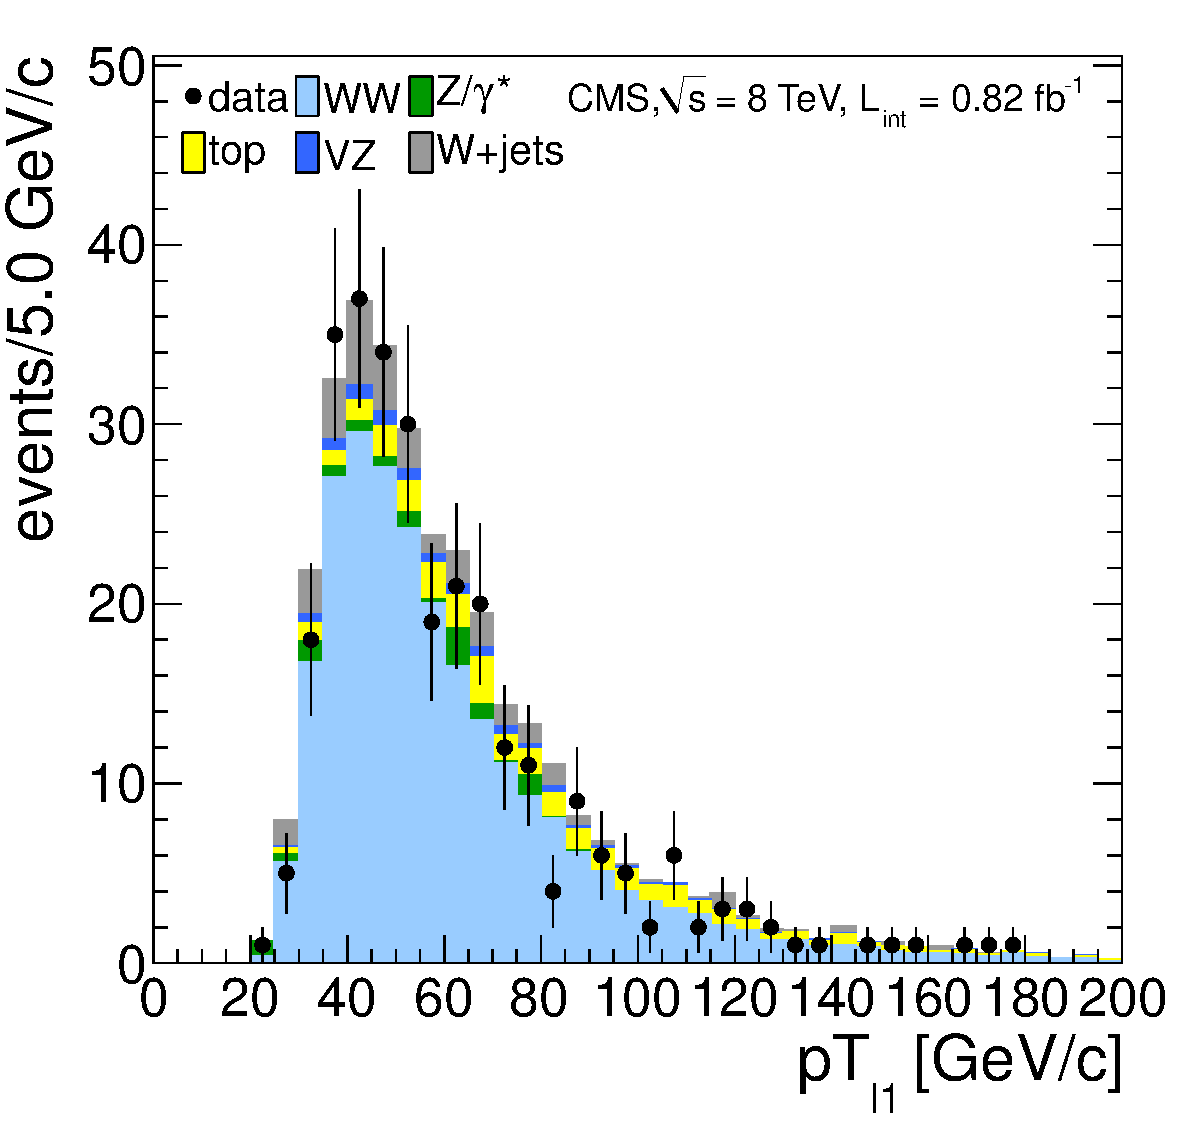
\includegraphics[width=.4\textwidth]{figures/lep1pt_mh0_nj0.pdf}
}
\subfigure[]{
\centering
\label{subfig:ww_ptmin_1j}
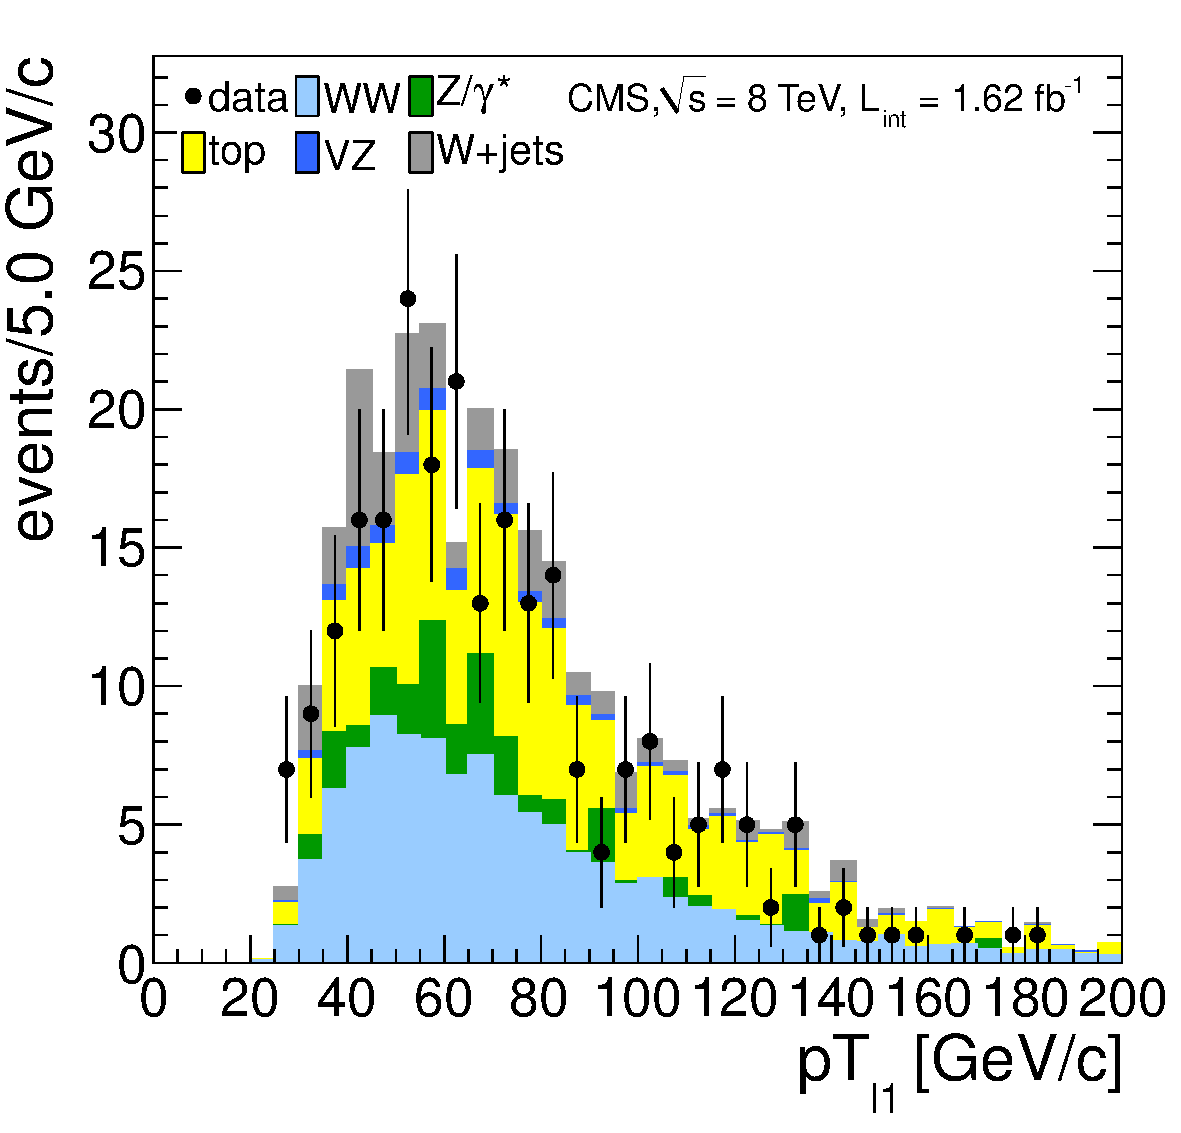
\includegraphics[width=.4\textwidth]{figures/lep1pt_mh0_nj1.pdf}
}
\subfigure[]{
\centering
\label{subfig:ww_ptmin_2j}
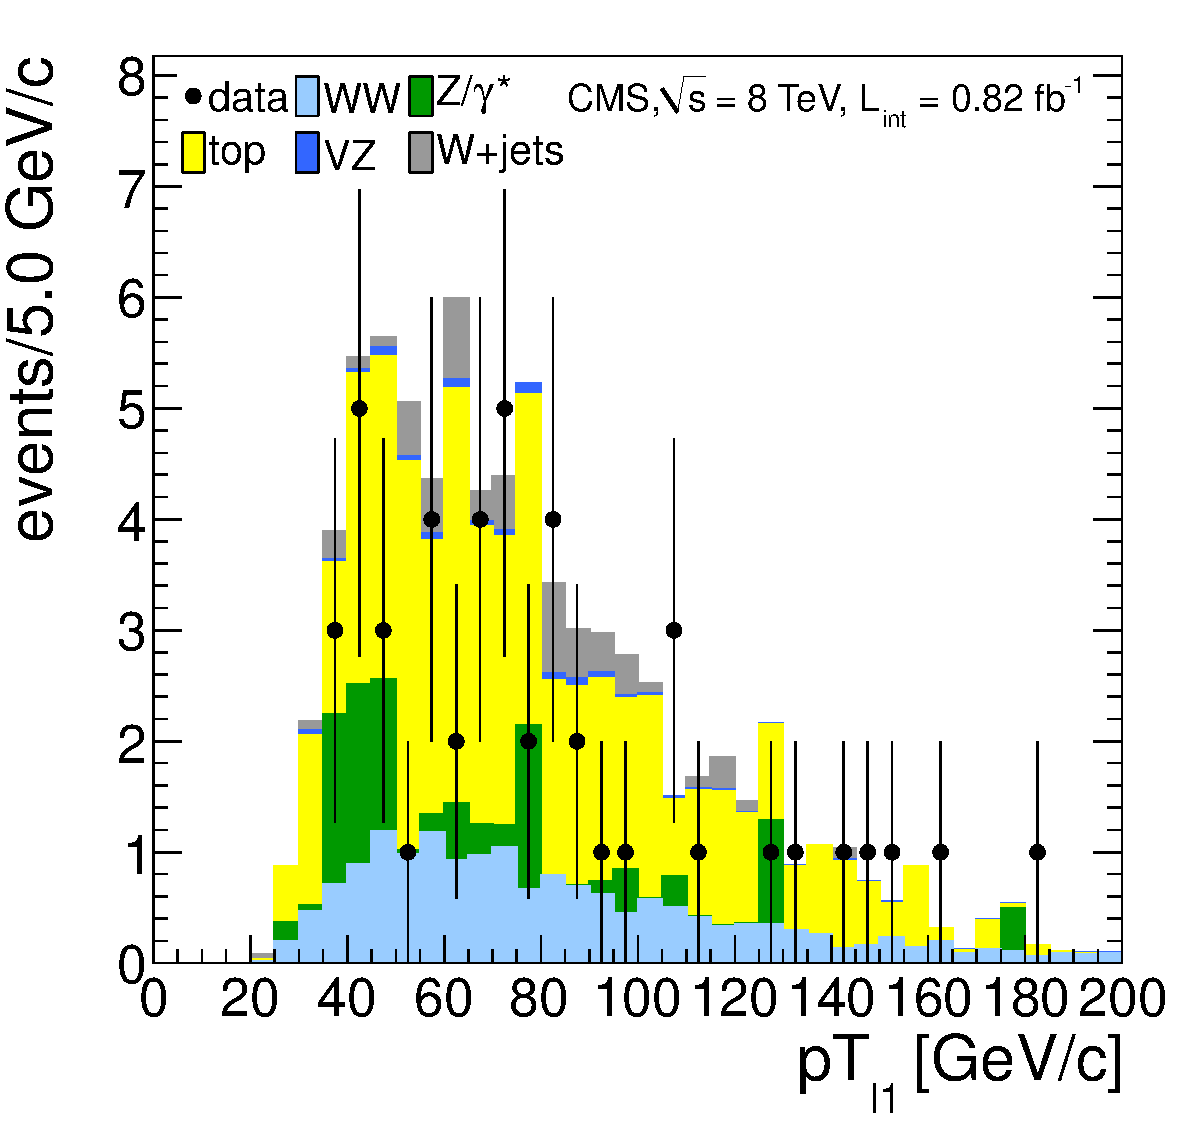
\includegraphics[width=.4\textwidth]{figures/lep1pt_mh0_nj2.pdf}
}
\caption{Trailing lepton $p_T$ distribution after WW selection for \intlumiEightTeV of data in the 0-jet \subref{subfig:ww_ptmin_0j}, 
1-jet \subref{subfig:ww_ptmin_1j} and 2-jet \subref{subfig:ww_ptmin_2j} bin analyses. 
MC is scaled to data-driven estimates.}
\label{fig:ww_ptmin}
\end{figure}

\begin{figure}[!hbtp]
\centering
\subfigure[]{
\centering
\label{subfig:ww_ptmax_0j}
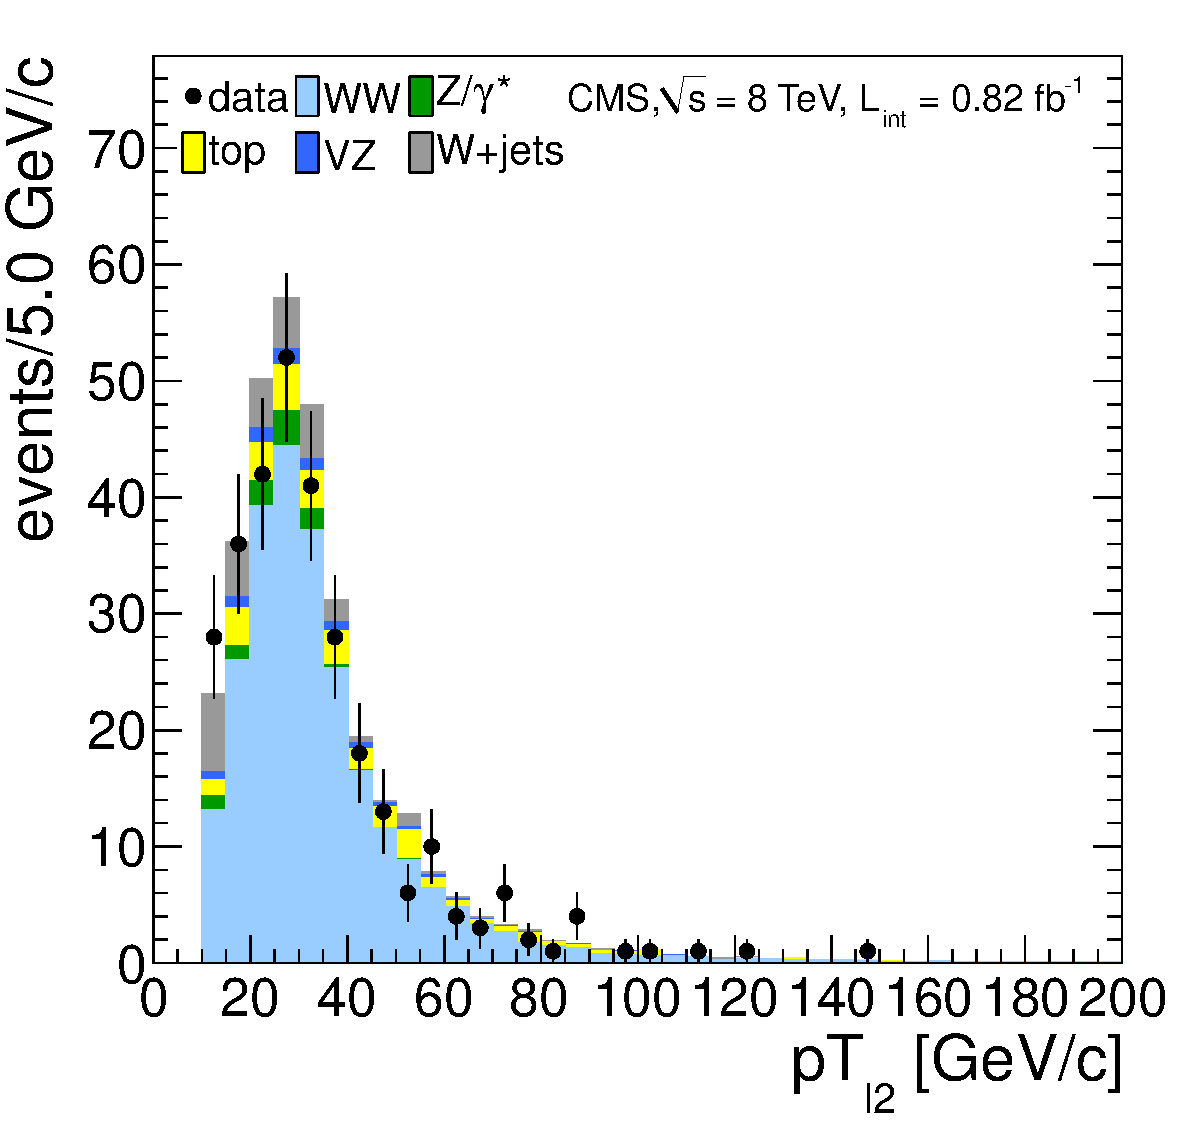
\includegraphics[width=.4\textwidth]{figures/lep2pt_mh0_nj0.pdf}
}
\subfigure[]{
\centering
\label{subfig:ww_ptmax_1j}
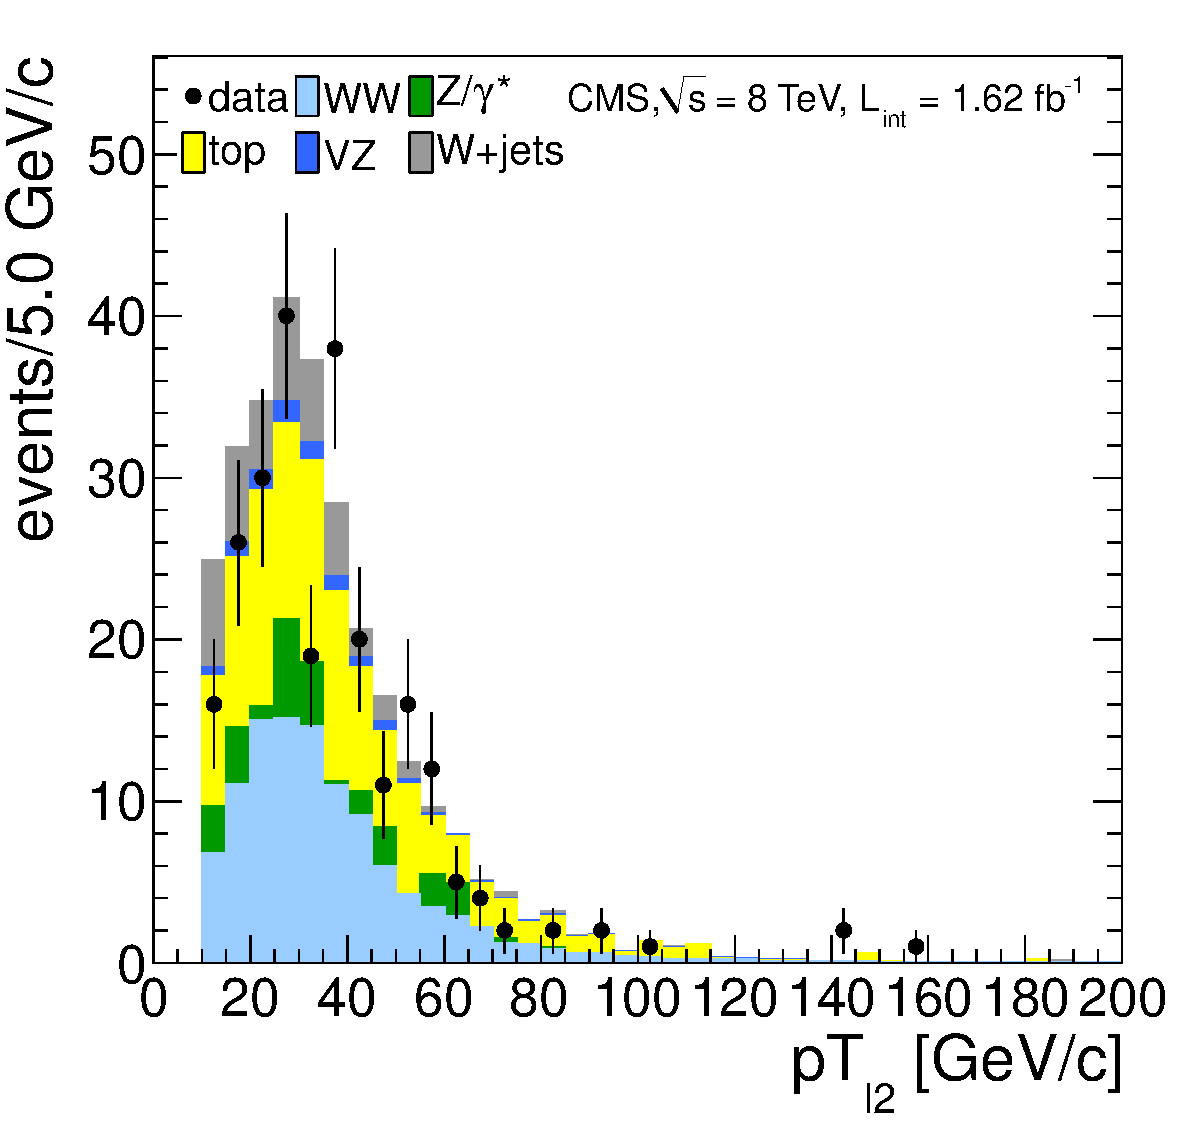
\includegraphics[width=.4\textwidth]{figures/lep2pt_mh0_nj1.pdf}
}
\subfigure[]{
\centering
\label{subfig:ww_ptmax_2j}
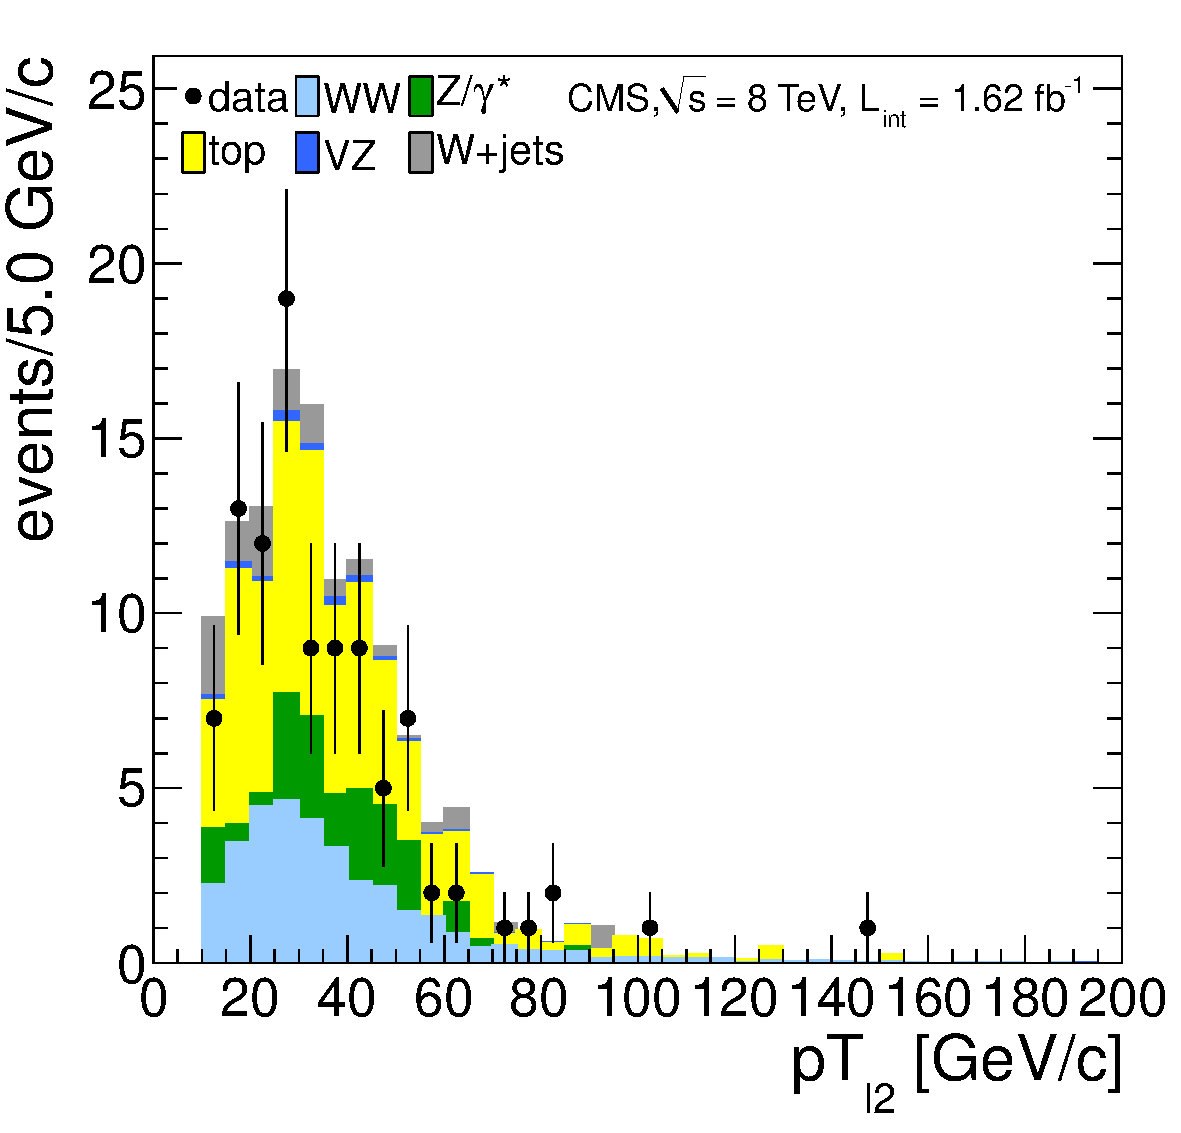
\includegraphics[width=.4\textwidth]{figures/lep2pt_mh0_nj2.pdf}
}\\
\caption{Leading lepton $p_T$ distribution after WW selection for \intlumiEightTeV of data in the 0-jet \subref{subfig:ww_ptmax_0j}, 
1-jet \subref{subfig:ww_ptmax_1j} and 2-jet \subref{subfig:ww_ptmax_2j} bin analyses. 
MC is scaled to data-driven estimates.}
\label{fig:ww_ptmax}
\end{figure}

\begin{figure}[!hbtp]
\centering
\subfigure[]{
\centering
\label{subfig:ww_pmet_0j}
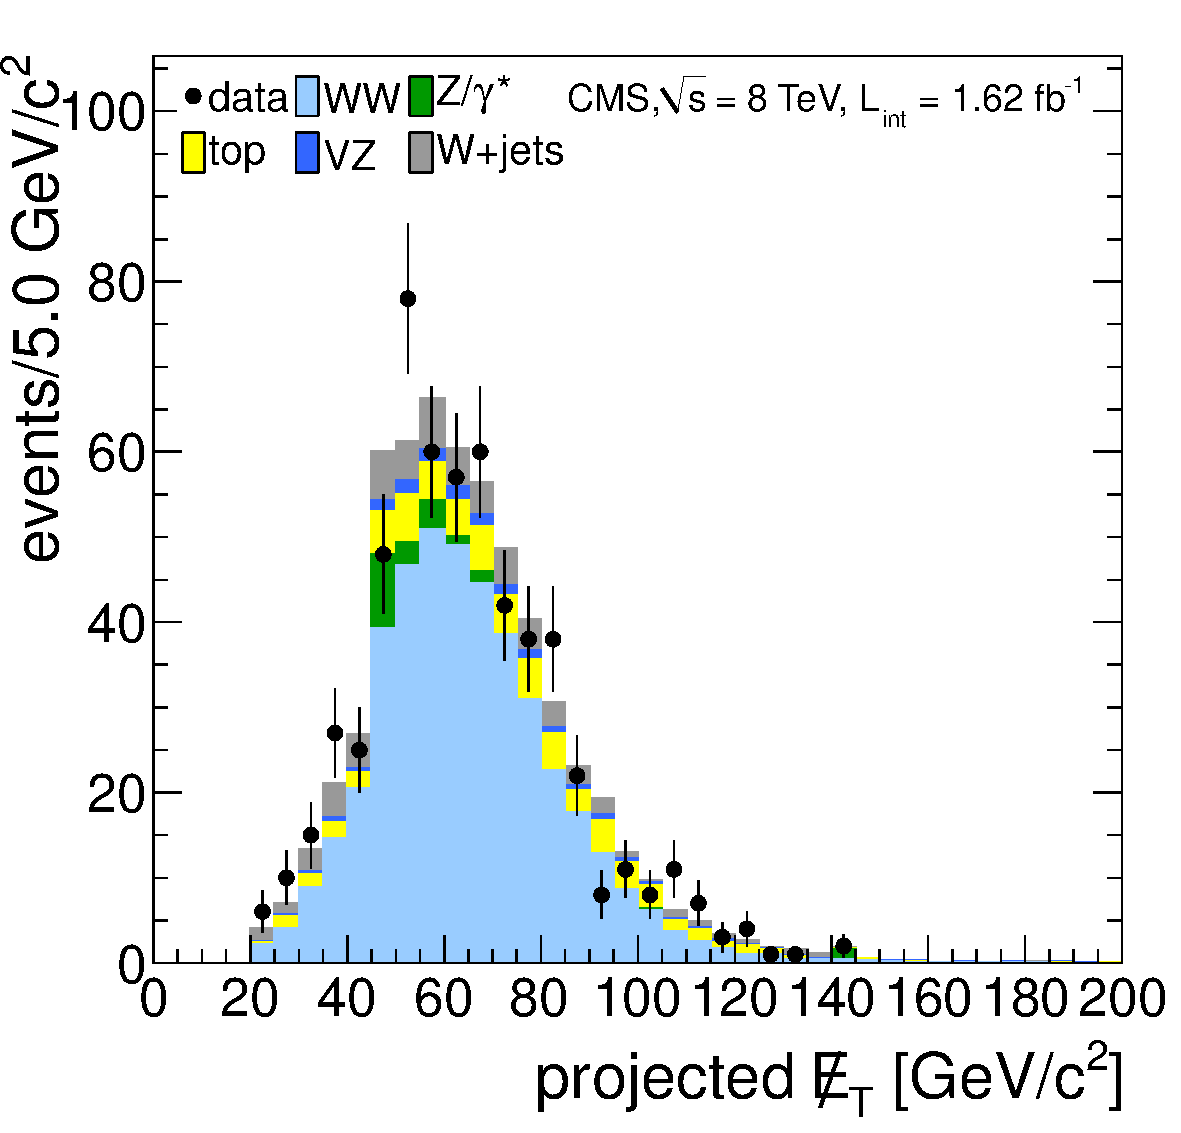
\includegraphics[width=.4\textwidth]{figures/pmet_mh0_nj0.pdf}
}
\subfigure[]{
\centering
\label{subfig:ww_pmet_1j}
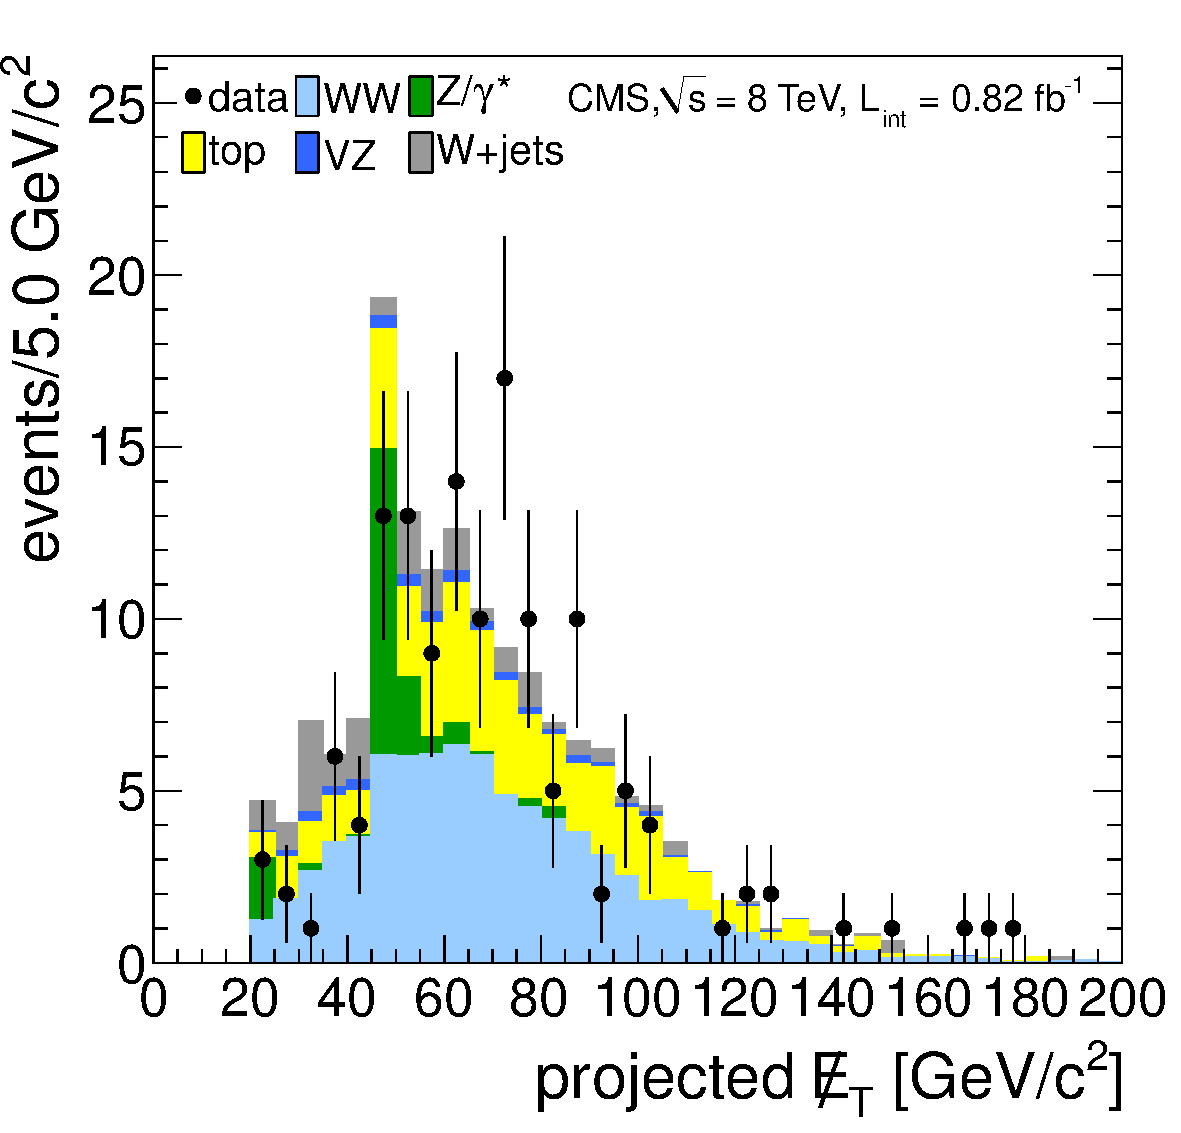
\includegraphics[width=.4\textwidth]{figures/pmet_mh0_nj1.pdf}
}
\subfigure[]{
\centering
\label{subfig:ww_pmet_2j}
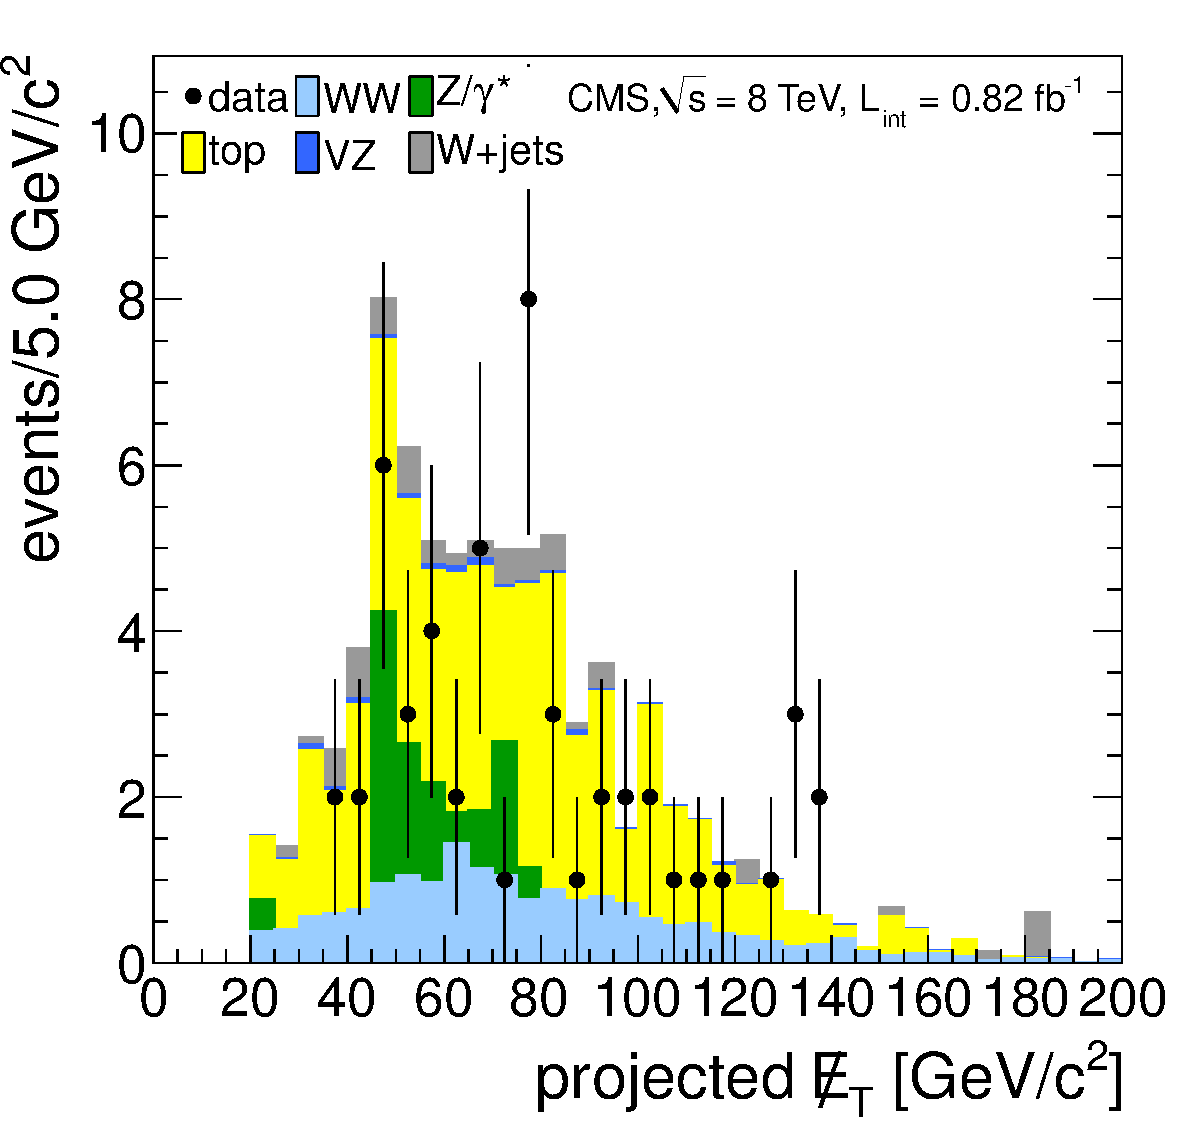
\includegraphics[width=.4\textwidth]{figures/pmet_mh0_nj2.pdf}
}\\
\caption{$min(\text{proj}_\text{trk-MET}, \text{proj}_\text{PFMET})$ distribution after WW selection for \intlumiEightTeV of data in the 0-jet \subref{subfig:ww_pmet_0j}, 
1-jet \subref{subfig:ww_pmet_1j} and 2-jet \subref{subfig:ww_pmet_2j} bin analyses. 
MC is scaled to data-driven estimates.}
\label{fig:ww_pmet}
\end{figure}

\begin{figure}[!hbtp]
\centering
\subfigure[]{
\centering
\label{subfig:ww_mt_0j}
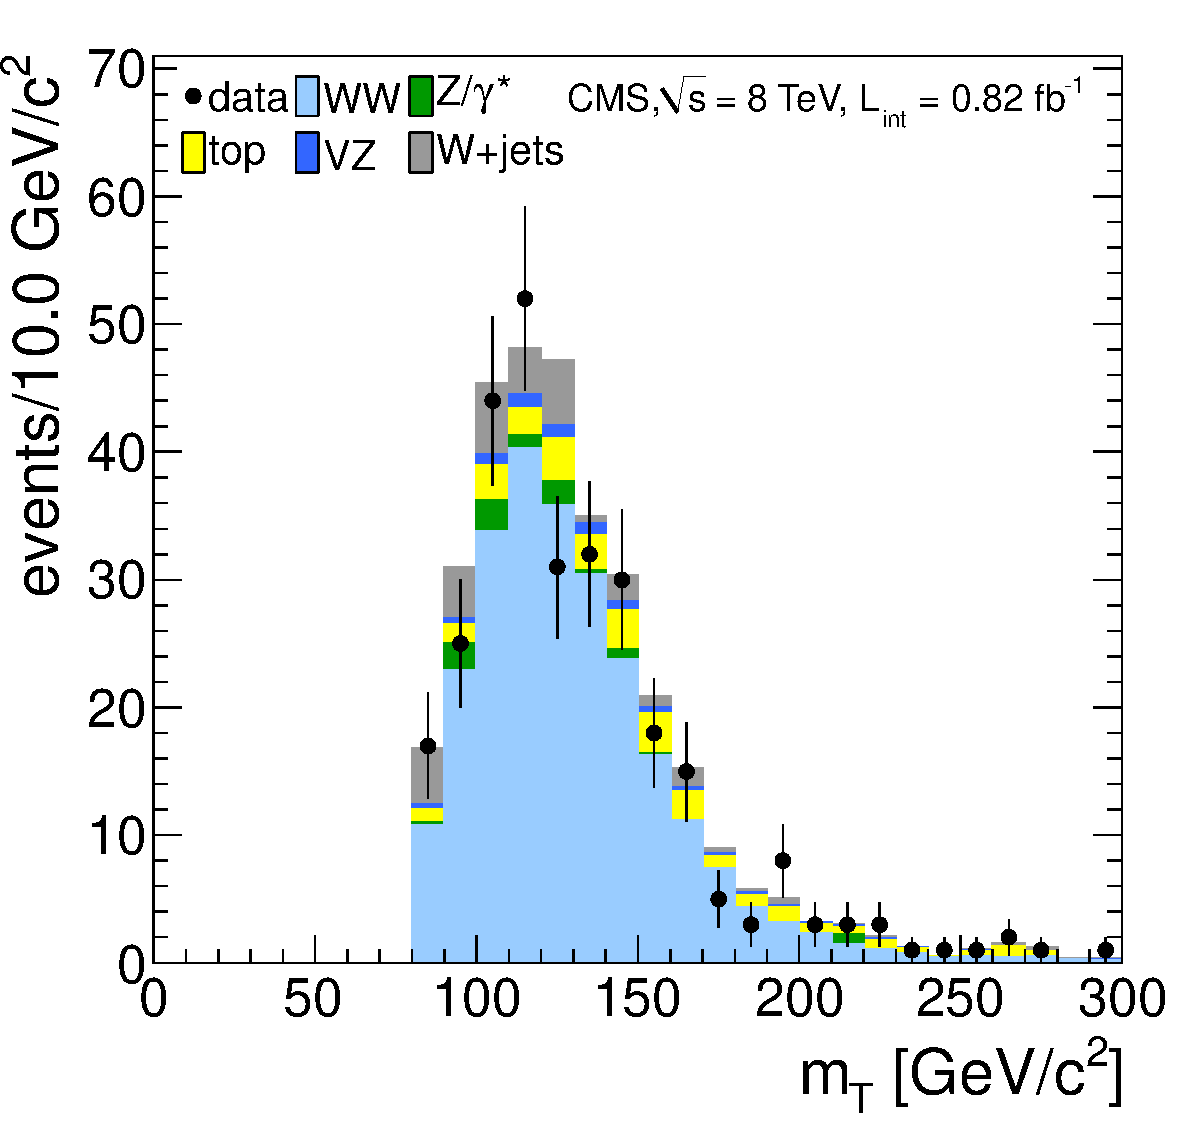
\includegraphics[width=.4\textwidth]{figures/mt_mh0_nj0.pdf}
}
\subfigure[]{
\centering
\label{subfig:ww_mt_1j}
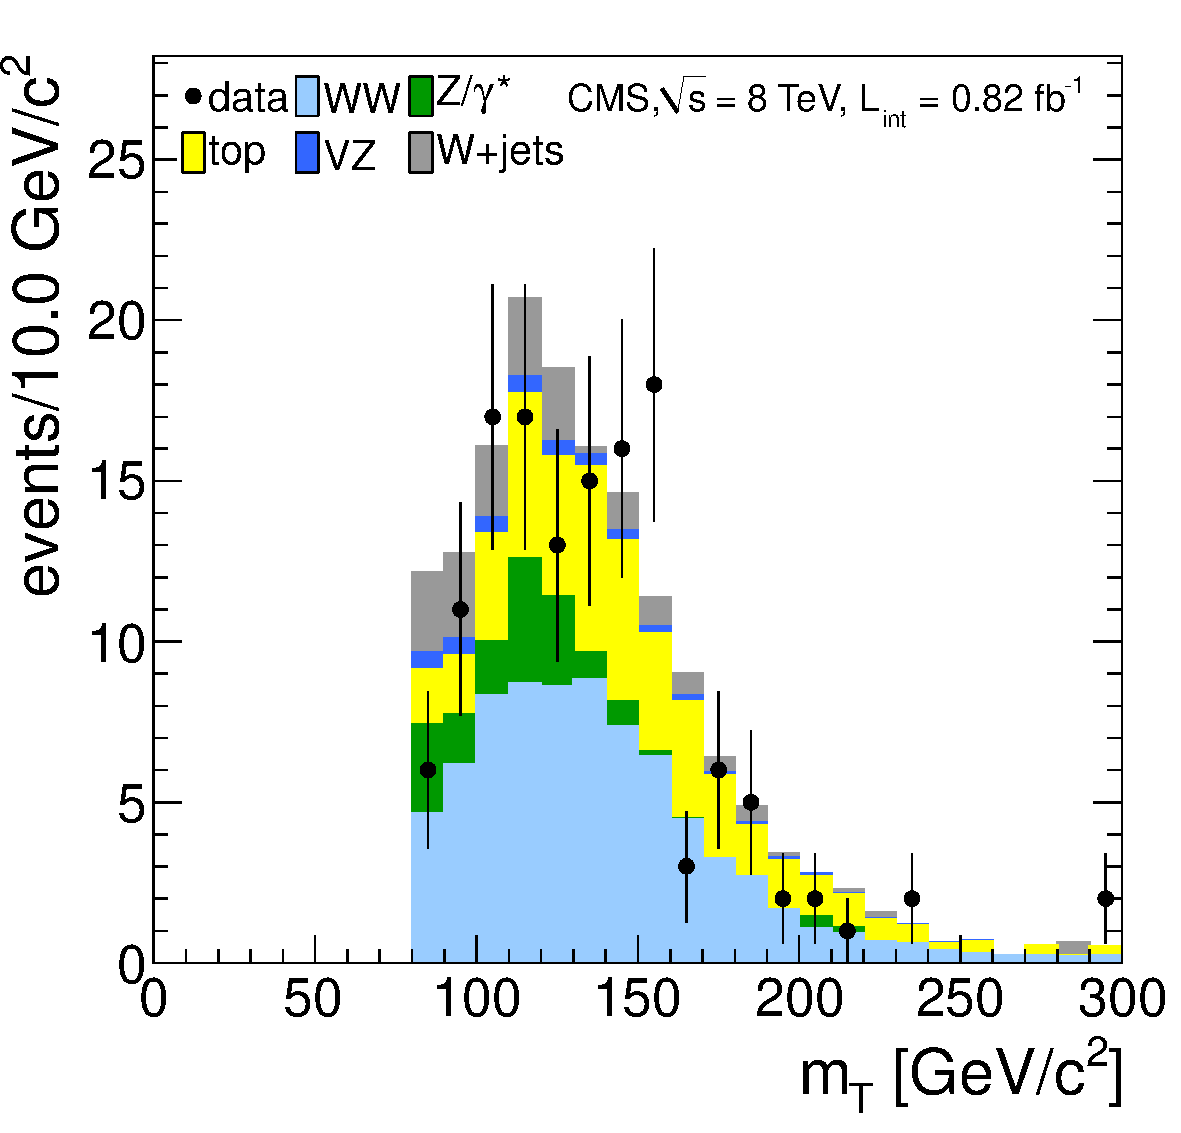
\includegraphics[width=.4\textwidth]{figures/mt_mh0_nj1.pdf}
}
\subfigure[]{
\centering
\label{subfig:ww_mt_2j}
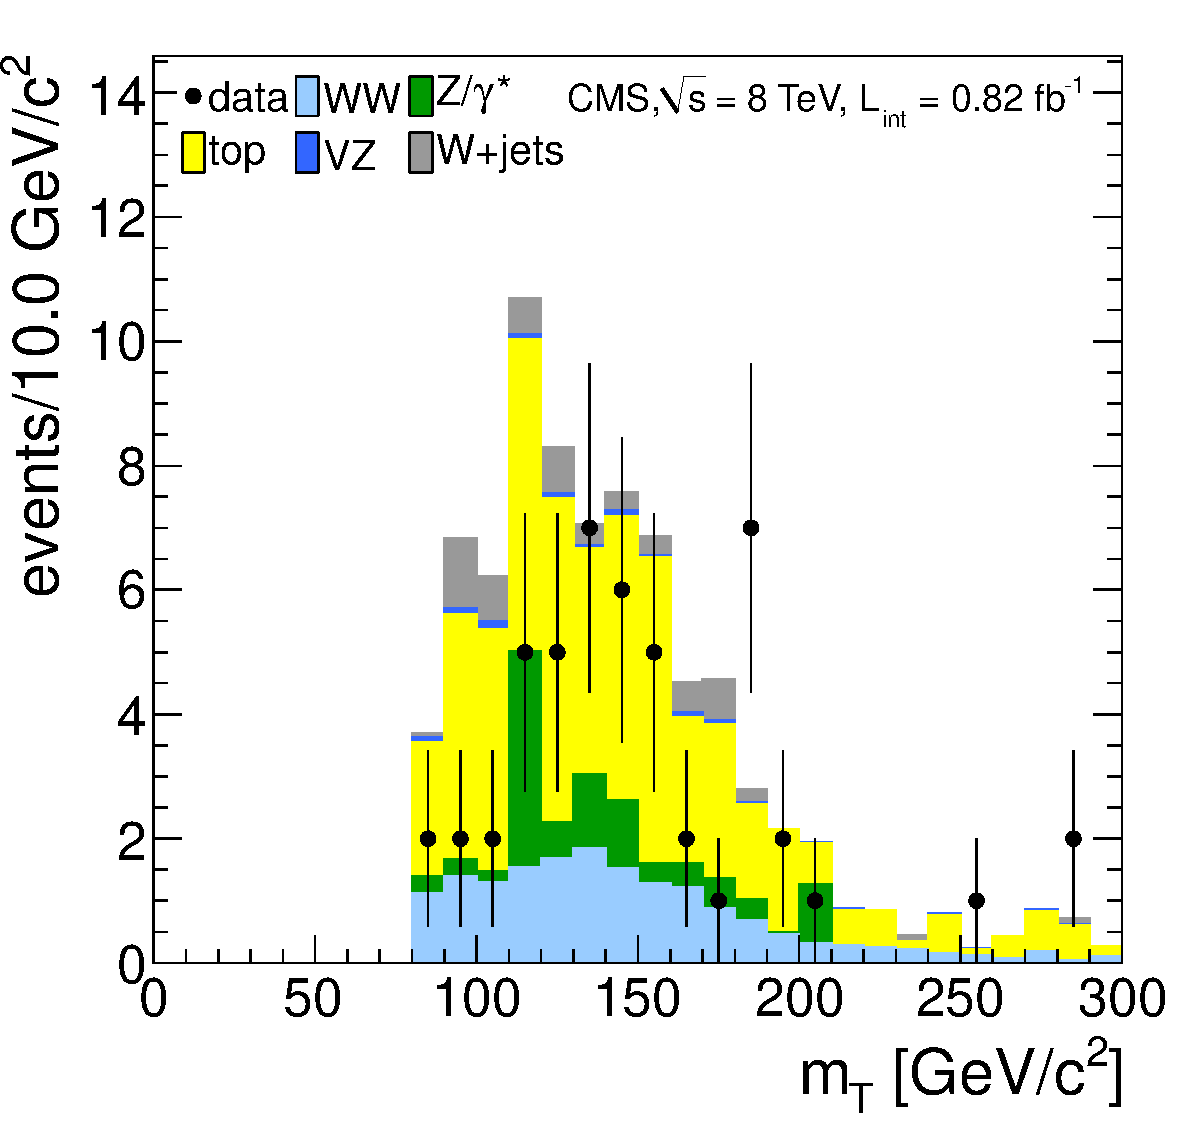
\includegraphics[width=.4\textwidth]{figures/mt_mh0_nj2.pdf}
} \\
\caption{Transverse mass distribution after WW selection for \intlumiEightTeV of data in the 0-jet \subref{subfig:ww_mt_0j}, 
1-jet \subref{subfig:ww_mt_1j} and 2-jet \subref{subfig:ww_mt_2j} bin analyses. 
MC is scaled to data-driven estimates.}
\label{fig:ww_mt}
\end{figure}

\begin{figure}[!hbtp]
\centering
\subfigure[]{
\centering
\label{subfig:ww_dilmass_0j}
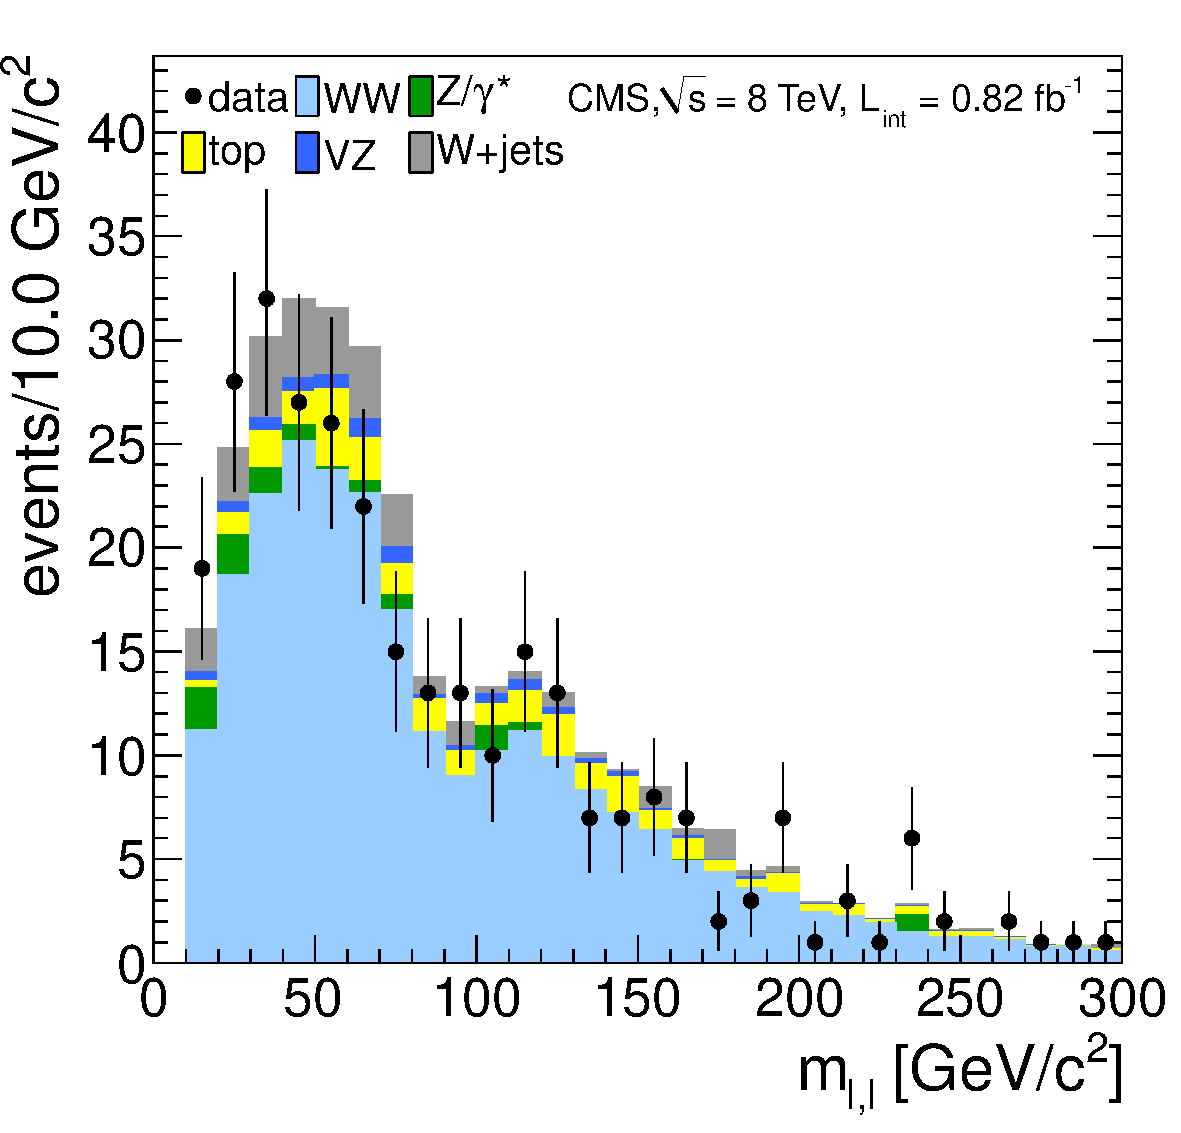
\includegraphics[width=.4\textwidth]{figures/dilepmass_mh0_nj0.pdf}
}
\subfigure[]{
\centering
\label{subfig:ww_dilmass_1j}
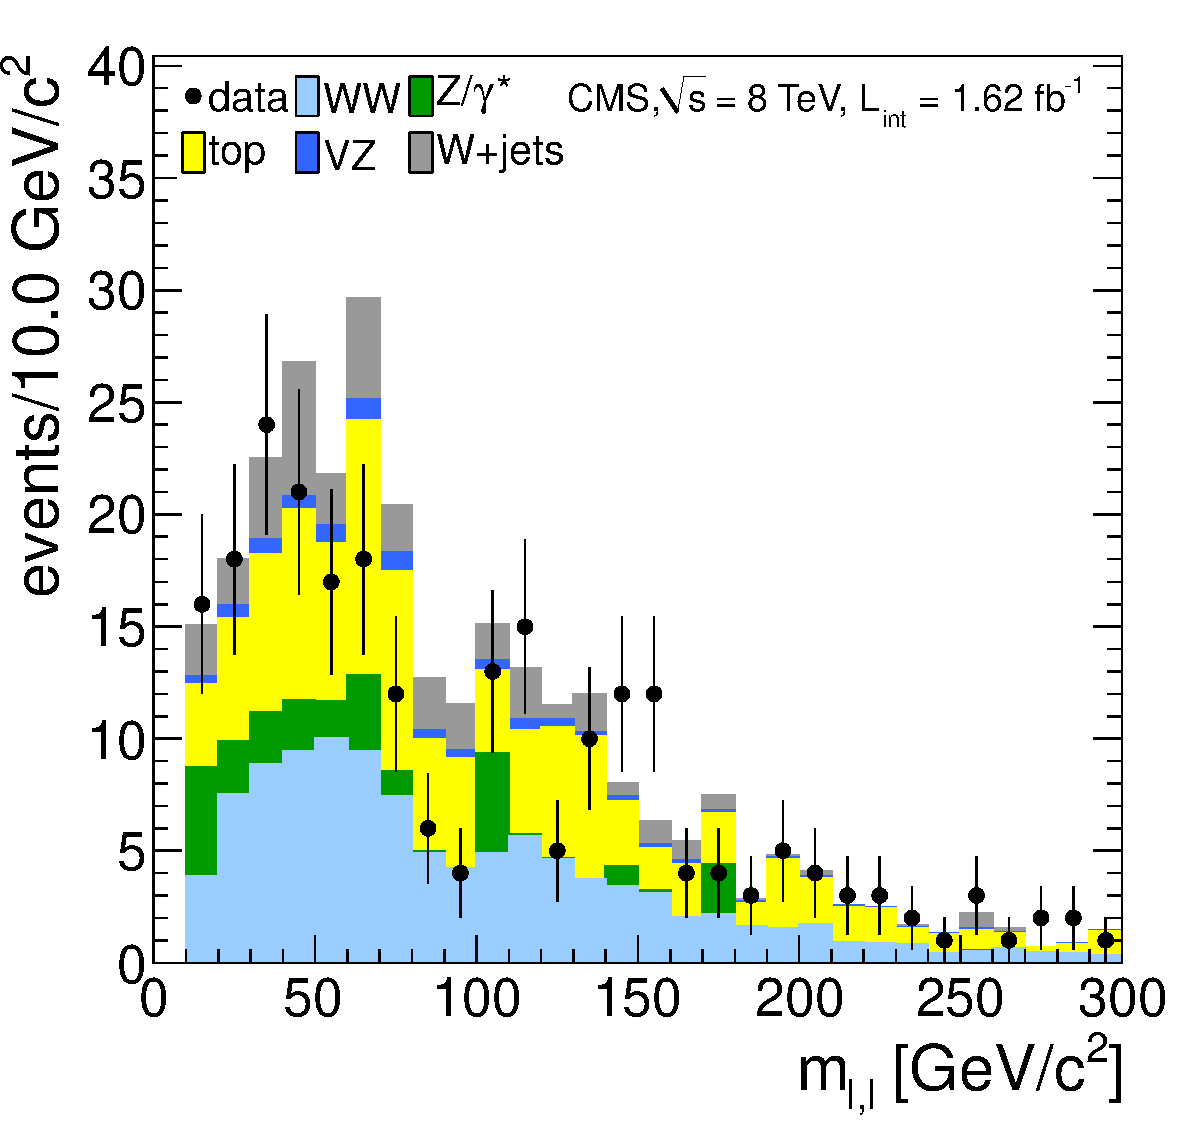
\includegraphics[width=.4\textwidth]{figures/dilepmass_mh0_nj1.pdf}
}
\subfigure[]{
\centering
\label{subfig:ww_dilmass_2j}
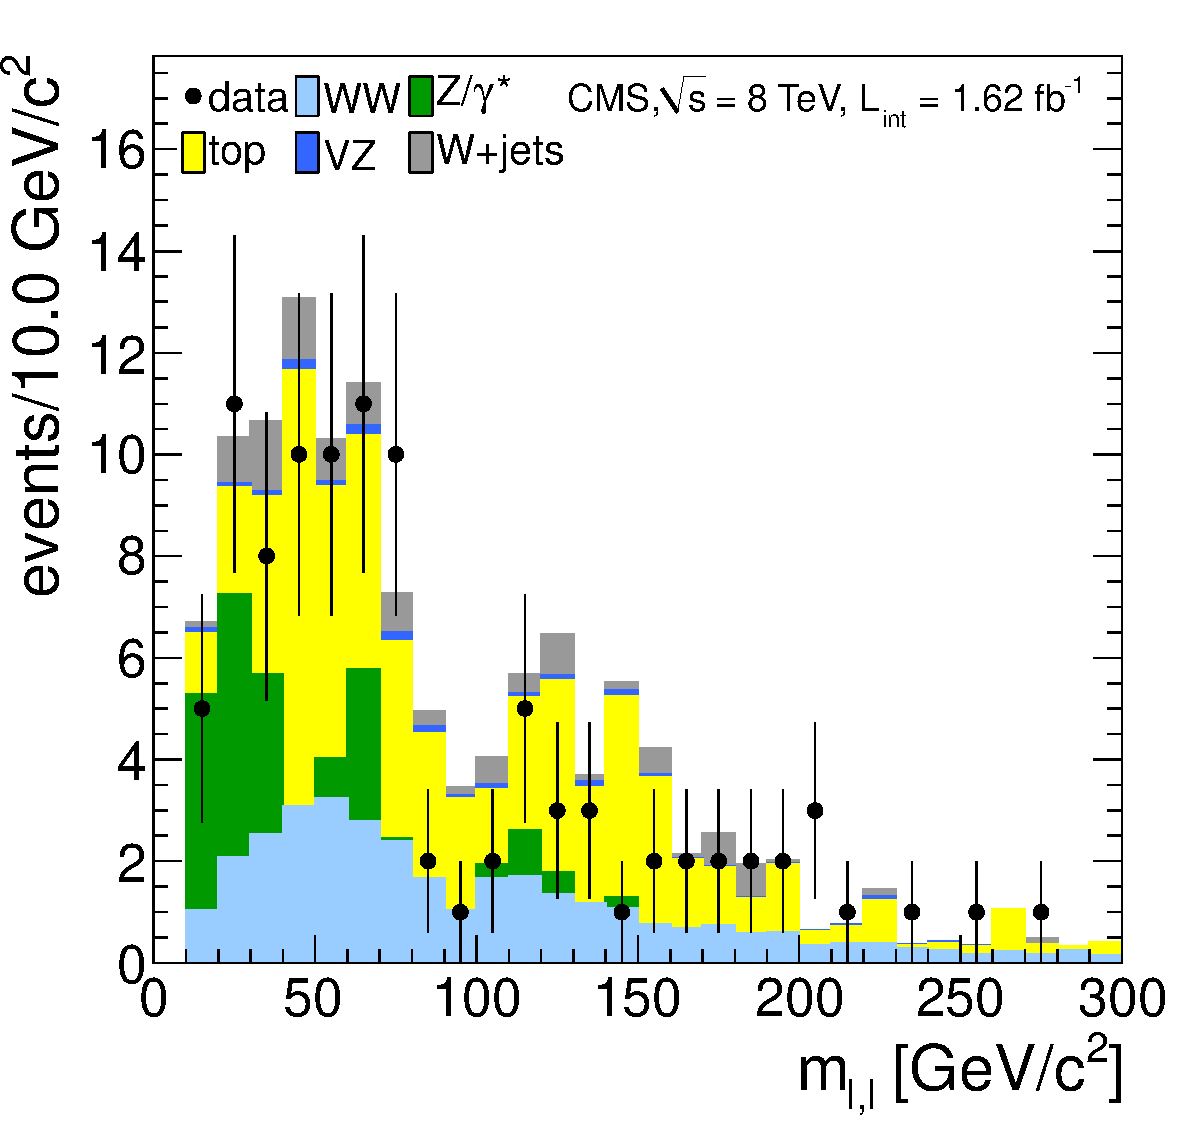
\includegraphics[width=.4\textwidth]{figures/dilepmass_mh0_nj2.pdf}
} \\
\caption{Invariant dilepton mass distribution after WW selection for \intlumiEightTeV of data in the 0-jet \subref{subfig:ww_dilmass_0j}, 
1-jet \subref{subfig:ww_dilmass_1j} and 2-jet \subref{subfig:ww_dilmass_2j} bin analyses. 
MC is scaled to data-driven estimates.}
\label{fig:ww_dilmass}
\end{figure}

\begin{figure}[!hbtp]
\centering
\subfigure[]{
\centering
\label{subfig:ww_deltaphi_0j}
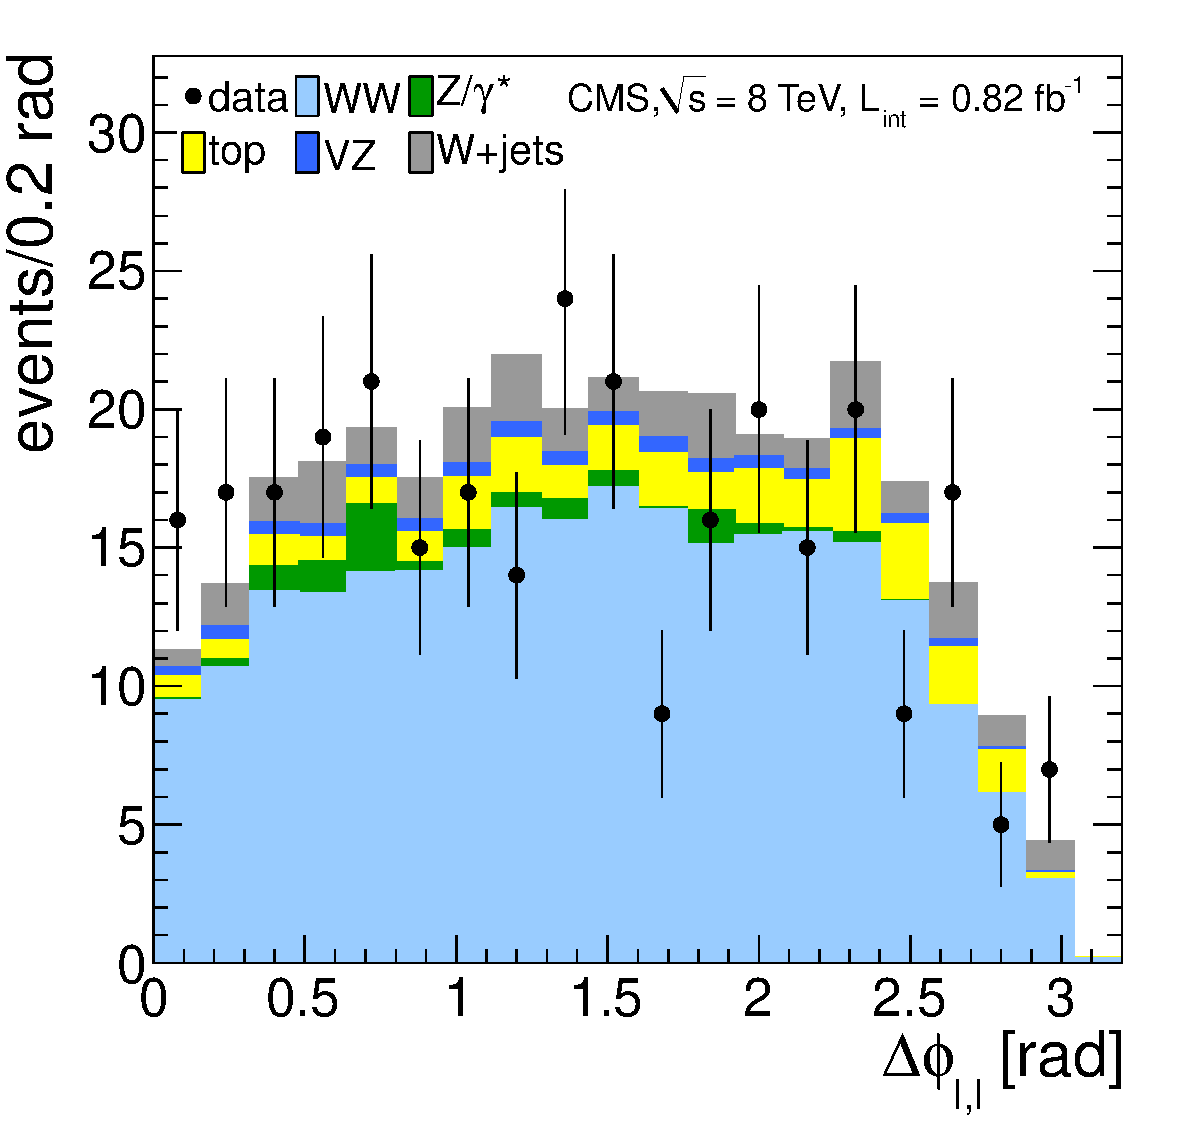
\includegraphics[width=.4\textwidth]{figures/dPhi_mh0_nj0.pdf}
}
\subfigure[]{
\centering
\label{subfig:ww_deltaphi_1j}
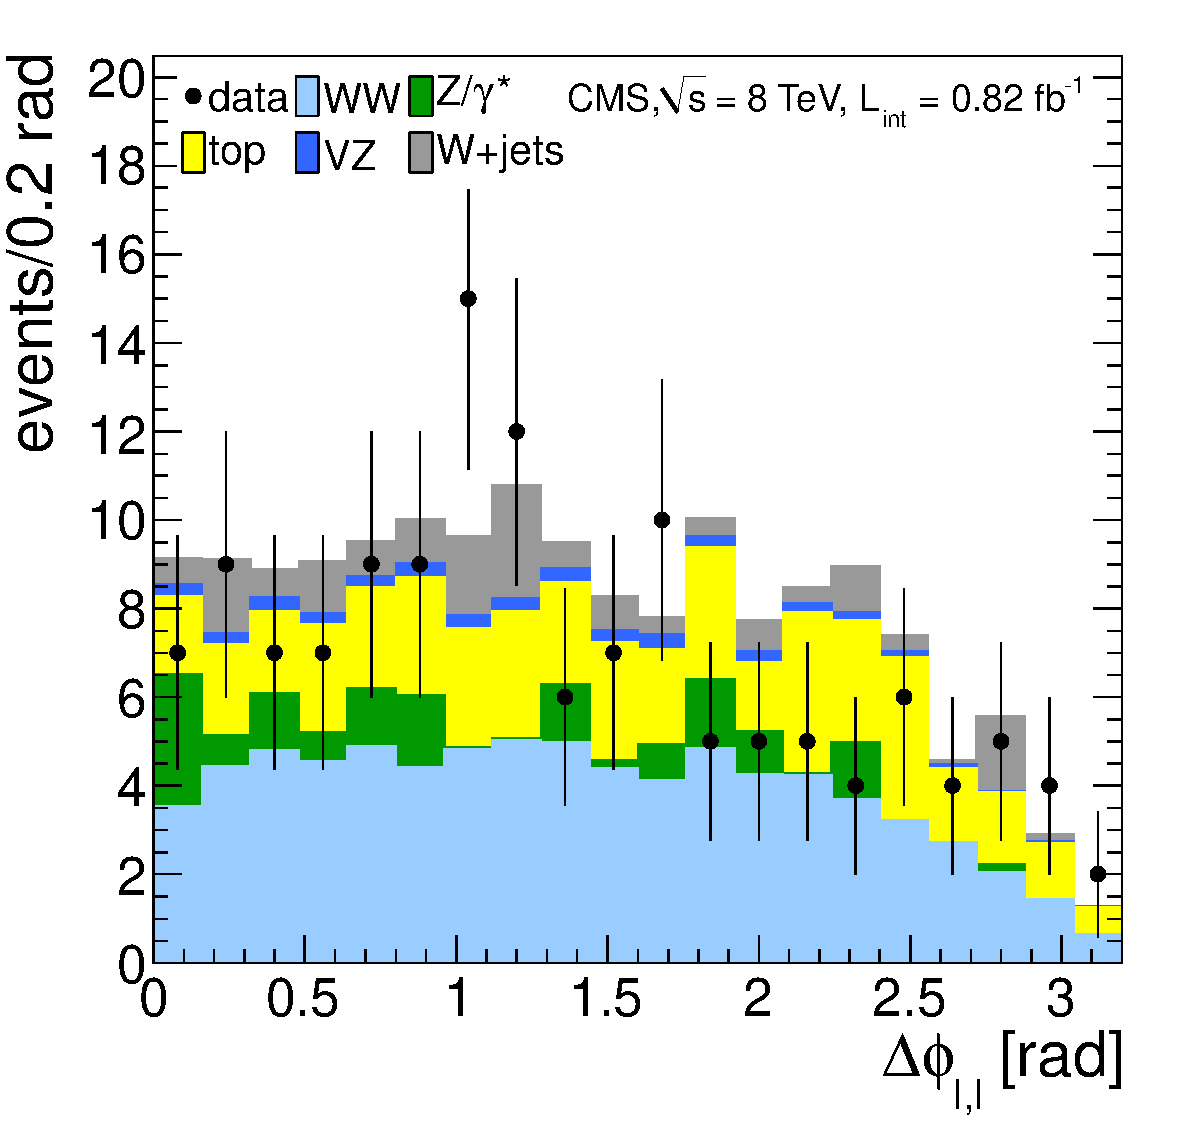
\includegraphics[width=.4\textwidth]{figures/dPhi_mh0_nj1.pdf}
}
\subfigure[]{
\centering
\label{subfig:ww_deltaphi_2j}
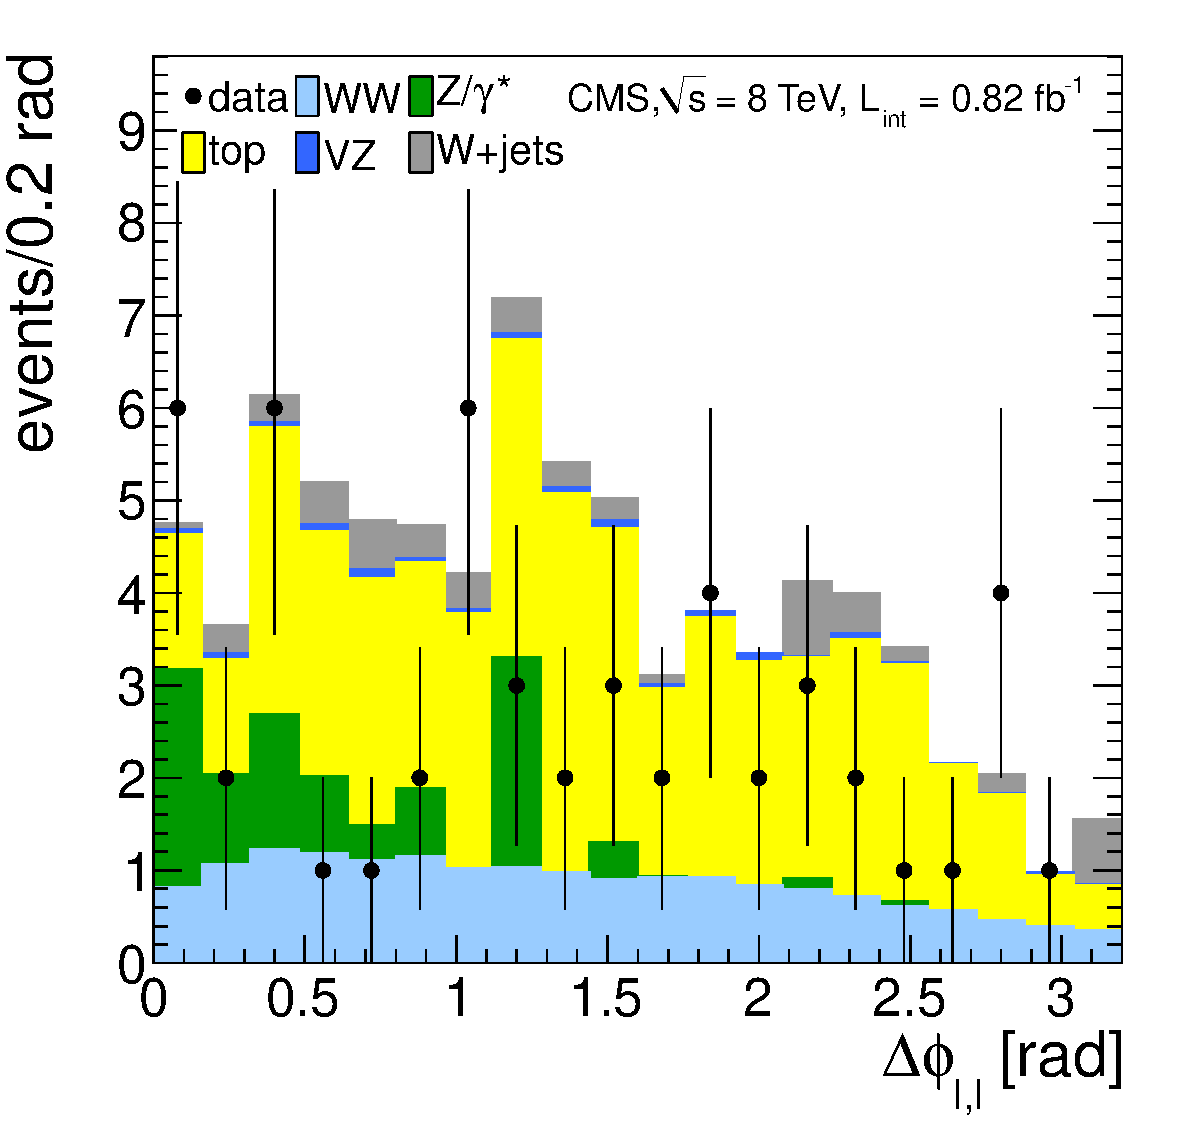
\includegraphics[width=.4\textwidth]{figures/dPhi_mh0_nj2.pdf}
} \\
\caption{Dilepton $\Delta\phi$ distribution after WW selection for \intlumiEightTeV of data in the 0-jet \subref{subfig:ww_deltaphi_0j}, 
1-jet \subref{subfig:ww_deltaphi_1j} and 2-jet \subref{subfig:ww_deltaphi_2j} bin analyses. 
MC is scaled to data-driven estimates.}
\label{fig:ww_deltaphi}
\end{figure}

\begin{table}[ht!]
\begin{center}
\begin{tabular}{c | c | c } 
\hline
              & \multicolumn{1}{c|}{0-jet} & \multicolumn{1}{c}{1-jet} \\
mass [\GeV] & scale factor & scale factor \\
\hline
115 &  1.37 $\pm$ 0.15 &  1.25 $\pm$ 0.27 \\
120 &  1.37 $\pm$ 0.15 &  1.25 $\pm$ 0.27 \\
130 &  1.37 $\pm$ 0.15 &  1.25 $\pm$ 0.27 \\
140 &  1.37 $\pm$ 0.15 &  1.25 $\pm$ 0.27 \\
150 &  1.15 $\pm$ 0.15 &  1.21 $\pm$ 0.27 \\
160 &  1.16 $\pm$ 0.15 &  1.03 $\pm$ 0.35 \\
170 &  1.16 $\pm$ 0.15 &  1.03 $\pm$ 0.35\\
180 &  1.13 $\pm$ 0.16 &  1.02 $\pm$ 0.35 \\
190 &  1.12 $\pm$ 0.16 &  1.02 $\pm$ 0.35 \\
\hline
\end{tabular}
\caption{WW background estimation for $\intlumiEightTeV$.}
\label{tab:ww_est}
\end{center}
\end{table}

%%%%%%%%%%%%%%%%%%%%%%%%%%%%%%
\subsection{Final Results for the Higgs Search with \intlumiEightTeV{}}
\label{sec:search_results}

The expected 
%and observed 
upper limits at 95\% C.L. for the cut based and
multivariate analyses are shown in Tables~\ref{tab:cutbase_uls}
and~\ref{tab:mvabase_uls}, respectively. The corresponding exclusion
limits are shown in Figure~\ref{fig:uls}. The detailed event yields 
for both analyses are summarized in Apps.~\ref{app:appendix_cutresults} 
and~\ref{app:appendix_bdtresults}.

\begin{figure}[!hbtp]
\centering
\subfigure[SM Higgs (cut-based)]{
\centering
\label{subfig:sm_cut}
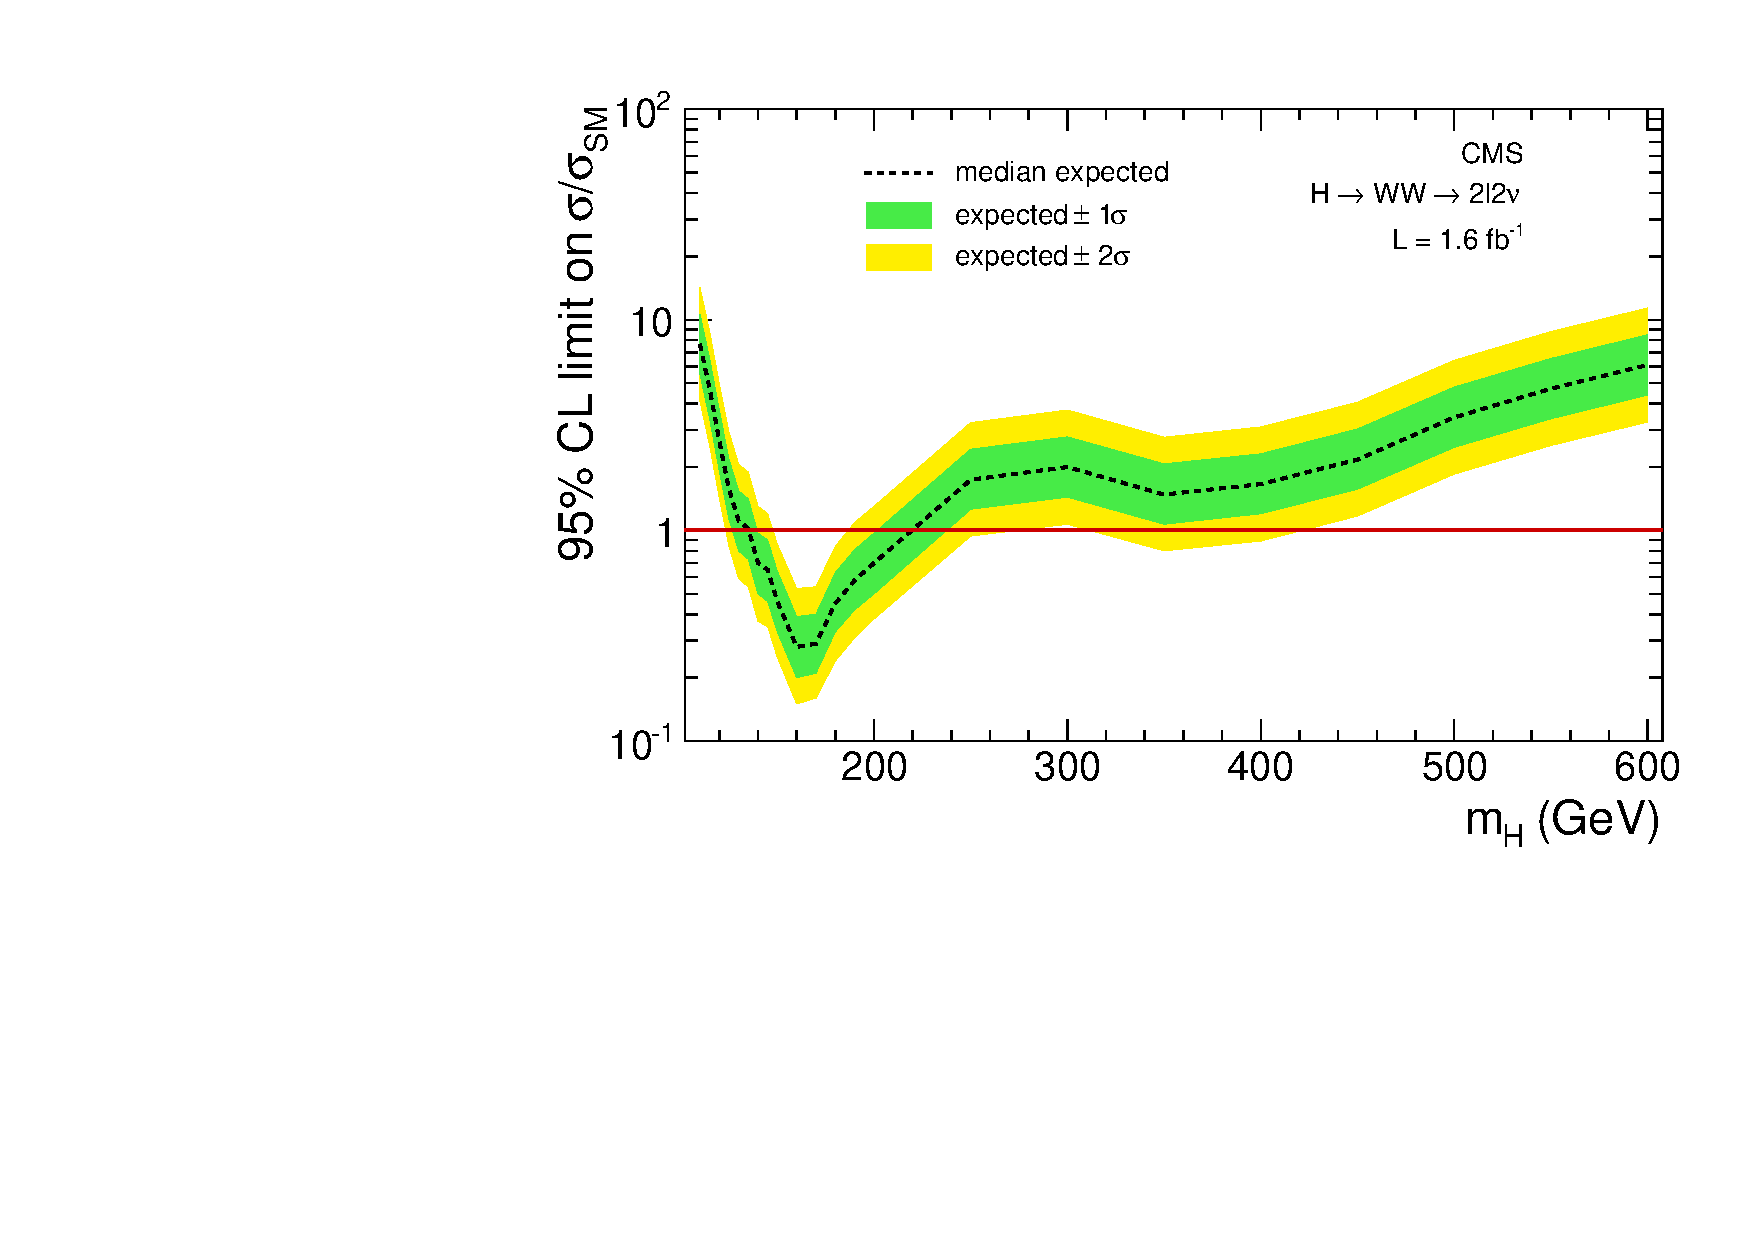
\includegraphics[width=.45\textwidth]{figures/limits_nj_cut_extended.pdf}
}
\subfigure[SM Higgs Zoomed (cut-based)]{
\centering
\label{subfig:sm_cut_zoom}
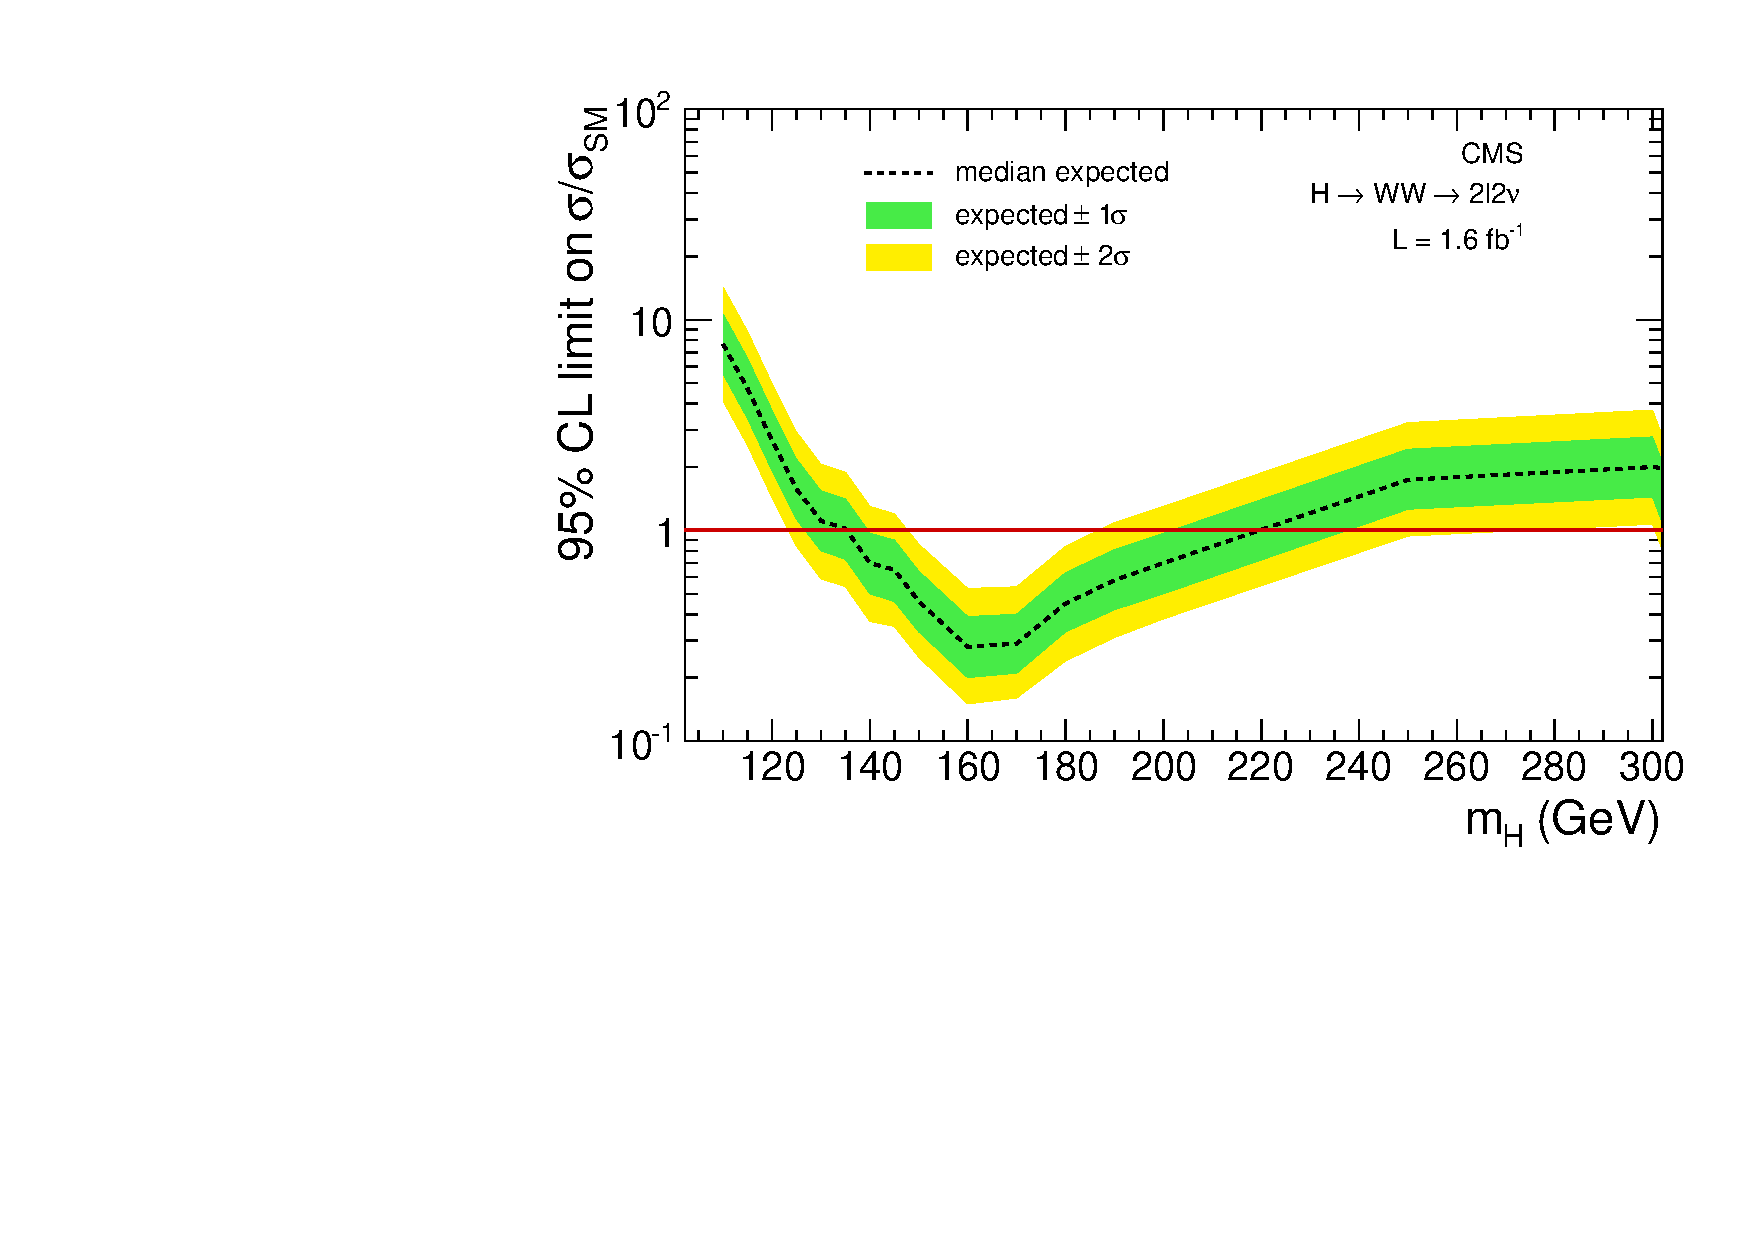
\includegraphics[width=.45\textwidth]{figures/limits_nj_cut.pdf}
}
\centering
\subfigure[SM Higgs (shape-based)]{
\centering
\label{subfig:sm_shape}
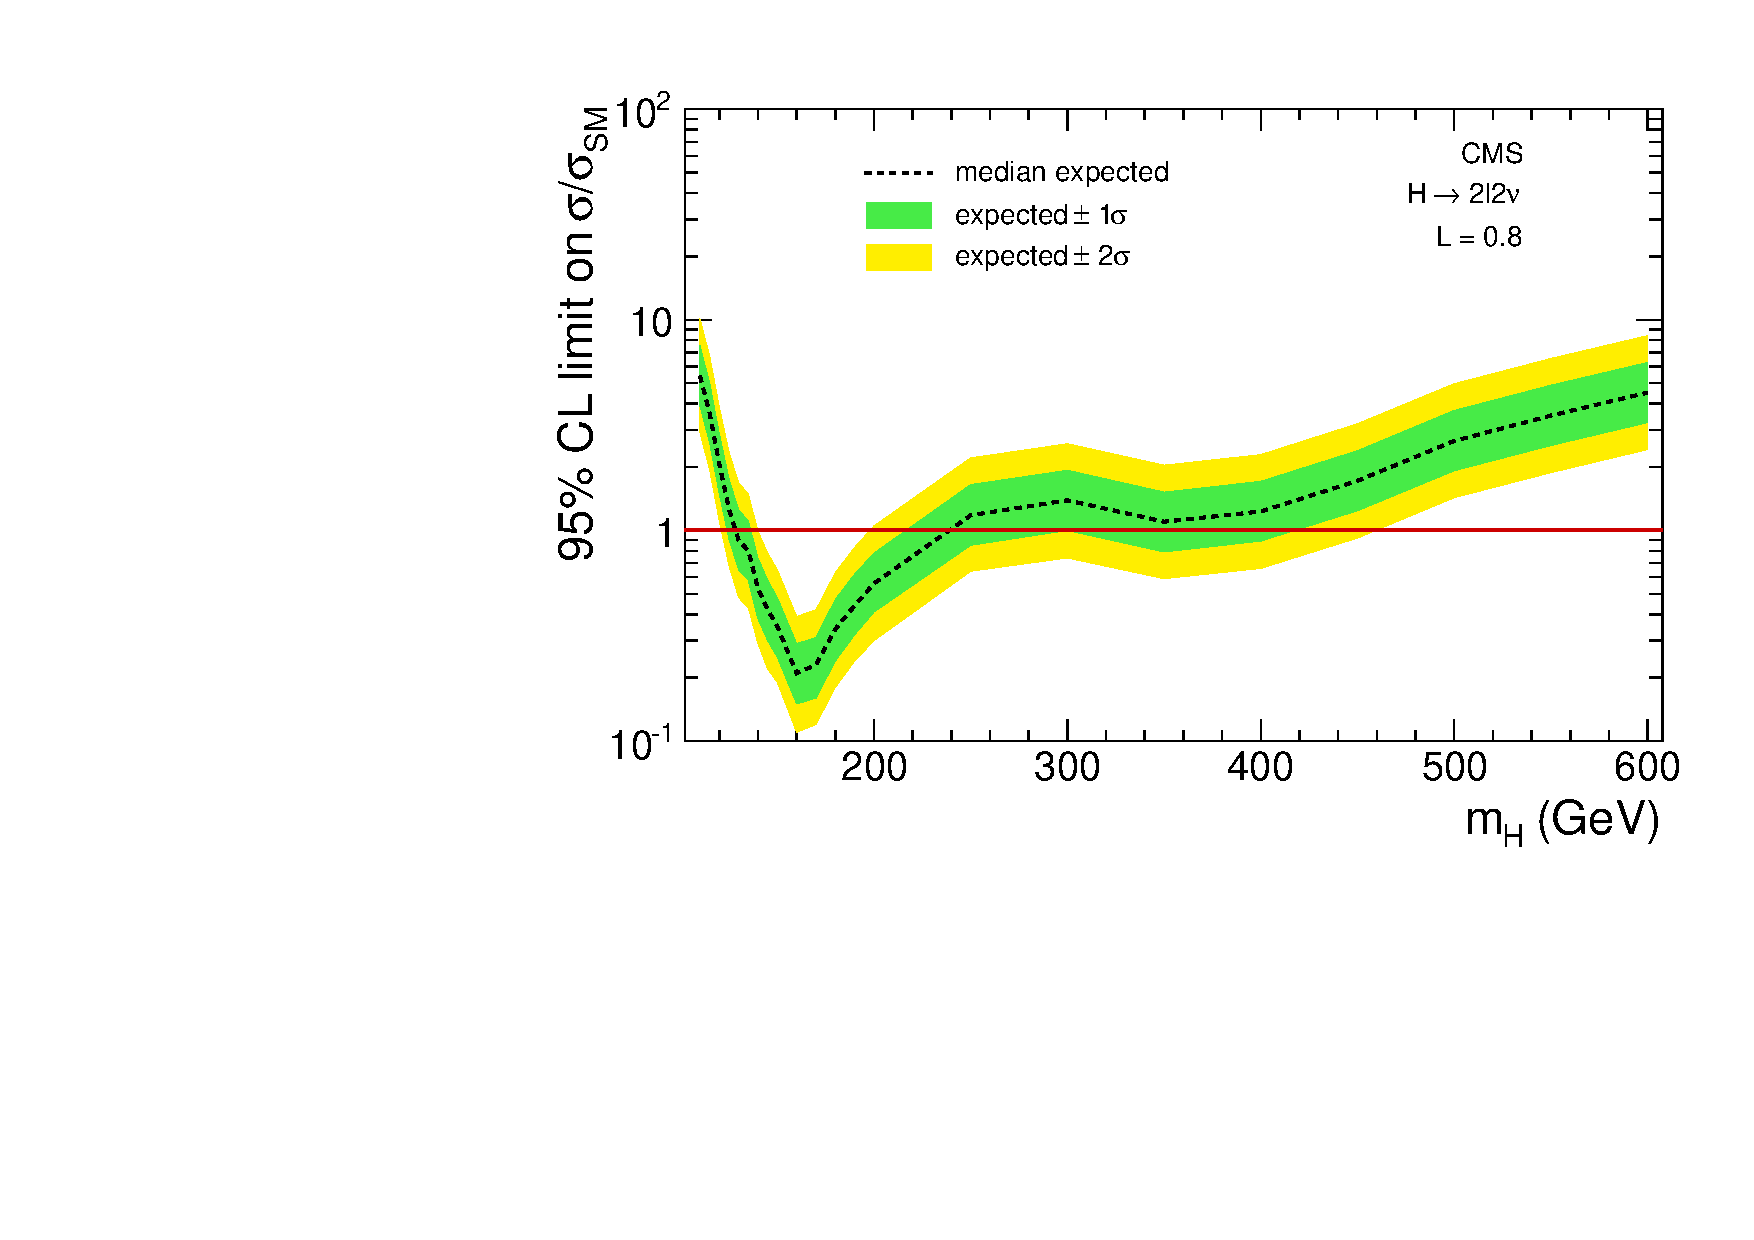
\includegraphics[width=.45\textwidth]{figures/limits_nj_shape_extended.pdf}
}
\subfigure[SM Higgs Zoomed (shape-based)]{
\centering
\label{subfig:sm_shape_zoom}
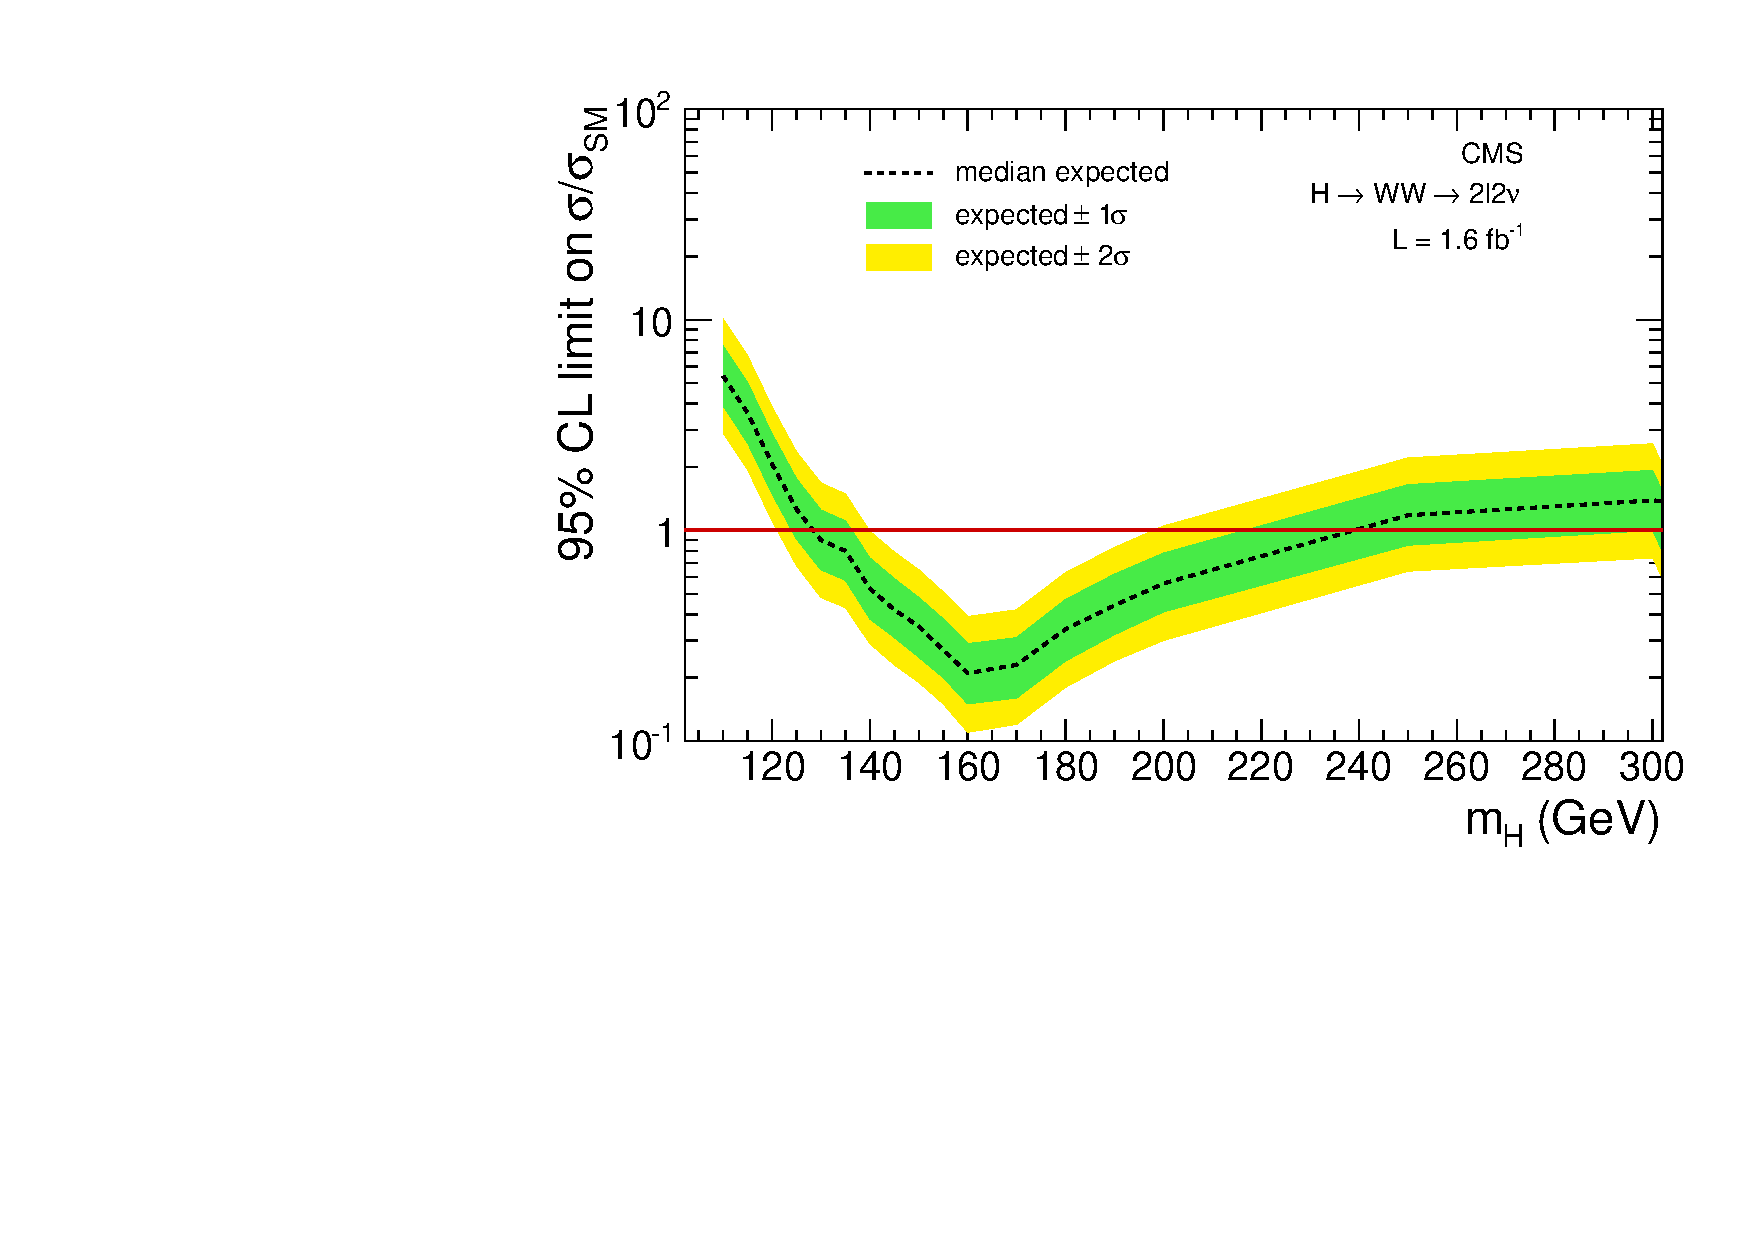
\includegraphics[width=.45\textwidth]{figures/limits_nj_shape.pdf}
}
\label{fig:uls}
\end{figure}

%%%%%%%%%%%%%%%%%%%%%%%%%%%%%%
\begin{table}[hbp!]
\begin{center}
\begin{tabular}{c c c c}
\hline
\vspace{-3mm} && \\
 Higgs Mass   & Median expected & Expected range for 68\% & Expected range for 95\%   \\
\vspace{-3mm} && \\
\hline
110 & 10.73 & [7.73, 14.93] & [5.76, 20.02] \\
115 &  6.45 & [4.64, 8.97] & [3.46, 12.02] \\ 
120 &  3.51 & [2.53, 4.89] & [1.88, 6.55] \\  
125 &  2.31 & [1.66, 3.22] & [1.24, 4.31] \\  
130 &  1.43 & [1.03, 1.99] & [0.77, 2.67] \\  
135 &  1.29 & [0.93, 1.79] & [0.69, 2.40] \\  
140 &  0.90 & [0.65, 1.26] & [0.48, 1.69] \\  
145 &  0.81 & [0.58, 1.12] & [0.43, 1.50] \\  
150 &  0.61 & [0.44, 0.84] & [0.33, 1.13] \\  
160 &  0.37 & [0.27, 0.52] & [0.20, 0.69] \\  
170 &  0.40 & [0.29, 0.56] & [0.22, 0.75] \\  
180 &  0.64 & [0.46, 0.88] & [0.34, 1.19] \\  
190 &  0.79 & [0.57, 1.10] & [0.43, 1.48] \\  
200 &  1.09 & [0.78, 1.51] & [0.58, 2.03] \\  
250 &  2.26 & [1.63, 3.14] & [1.21, 4.21] \\  
300 &  2.59 & [1.87, 3.61] & [1.39, 4.83] \\  
350 &  2.11 & [1.52, 2.93] & [1.13, 3.93] \\  
400 &  2.09 & [1.51, 2.91] & [1.12, 3.91] \\  
450 &  3.12 & [2.25, 4.34] & [1.67, 5.82] \\  
500 &  4.58 & [3.30, 6.37] & [2.46, 8.54] \\  
550 &  6.36 & [4.58, 8.84] & [3.41, 11.85] \\ 
600 &  8.28 & [5.96, 11.52] & [4.44, 15.44] \\
\hline
\end{tabular}
\caption{Expected and observed upper limits for SM Higgs using the
  {\bf cut-based} analysis with \intlumiEightTeV\ of data}
\label{tab:cutbase_uls}
\end{center}
\end{table}
%%%%%%%%%%%%%%%%%%%%%%%%%%%%%%

%%%%%%%%%%%%%%%%%%%%%%%%%%%%%%
\begin{table}[hbp!]
\begin{center}
\begin{tabular}{c c c c}
\hline
\vspace{-3mm} && \\
 Higgs Mass   & Median expected & Expected range for 68\% & Expected range for 95\%   \\
\vspace{-3mm} && \\
\hline
110 & 8.07 & [5.81, 11.22] & [4.33, 15.05] \\ 
115 & 4.86 & [3.50, 6.77] & [2.61, 9.07] \\   
120 & 2.97 & [2.14, 4.13] & [1.59, 5.54] \\   
125 & 1.94 & [1.40, 2.70] & [1.04, 3.62] \\   
130 & 1.21 & [0.87, 1.68] & [0.65, 2.25] \\   
135 & 1.03 & [0.74, 1.44] & [0.55, 1.93] \\   
140 & 0.73 & [0.53, 1.02] & [0.39, 1.36] \\   
145 & 0.58 & [0.42, 0.80] & [0.31, 1.07] \\   
150 & 0.47 & [0.34, 0.66] & [0.25, 0.88] \\   
160 & 0.28 & [0.20, 0.39] & [0.15, 0.52] \\   
170 & 0.30 & [0.22, 0.42] & [0.16, 0.57] \\   
180 & 0.48 & [0.34, 0.66] & [0.26, 0.89] \\   
190 & 0.61 & [0.44, 0.85] & [0.33, 1.14] \\   
200 & 0.86 & [0.62, 1.19] & [0.46, 1.60] \\   
250 & 1.60 & [1.15, 2.23] & [0.86, 2.99] \\   
300 & 1.88 & [1.36, 2.62] & [1.01, 3.51] \\   
350 & 1.67 & [1.20, 2.33] & [0.90, 3.12] \\   
400 & 1.70 & [1.22, 2.37] & [0.91, 3.17] \\   
450 & 2.52 & [1.81, 3.50] & [1.35, 4.70] \\   
500 & 3.67 & [2.64, 5.10] & [1.97, 6.84] \\   
550 & 5.02 & [3.61, 6.98] & [2.69, 9.36] \\   
600 & 6.24 & [4.50, 8.68] & [3.35, 11.64] \\  
\hline
\end{tabular}
\caption{Expected and observed upper limits for SM Higgs using the
  {\bf shape-based} analysis with \intlumiEightTeV\ of data}
\label{tab:mvabase_uls}
\end{center}
\end{table}
%%%%%%%%%%%%%%%%%%%%%%%%%%%%%%
